% !TeX program = xelatex
% !TeX encoding = UTF-8
% !TeX spellcheck = en_US
% !BIB program = biber
%%
%% Master thesis: Lizard on Llama-3.2-1B
%% Layout: the JKU LaTeX thesis template (jkureport.sty) by Michael Roland,
%% https://github.com/michaelroland/jku-templates-report-latex, MPL-2.0 (see JKU-TEMPLATE-LICENSE.txt).
%% Build: make (XeLaTeX and biber through latexmk). Output: thesis.pdf, copied to ../thesis.pdf
%%
\documentclass[a4paper,oneside,10pt,ngerman,english]{scrbook}

\usepackage[mathesis,fancyfonts,mathastext]{jkureport}
%% The template uses the JKU (gray) color scheme by default.
%% The option TNF selects the color scheme of the Faculty of Engineering and Natural Sciences.

% Preamble of the thesis
\usepackage[T1]{fontenc}
\usepackage[utf8]{inputenc}
\usepackage{lmodern}
\usepackage[english]{babel}
\usepackage{microtype}
\usepackage[a4paper,left=3cm,right=2.5cm,top=2.5cm,bottom=2.5cm,headheight=15pt]{geometry}
\usepackage{setspace}
\onehalfspacing

\usepackage{amsmath,amssymb,bm}
\usepackage{graphicx}
\usepackage{xcolor}
\usepackage{booktabs,tabularx,longtable,multirow,makecell,array}
\usepackage{caption,subcaption}
\usepackage{float}
\usepackage{enumitem}
\usepackage{titlesec}
\usepackage{fancyhdr}
\usepackage{csquotes}
\usepackage[numbers,sort&compress]{natbib}
\usepackage{xurl}
\usepackage{tikz}
\usetikzlibrary{arrows.meta,positioning,fit,calc,backgrounds}
\usepackage[most]{tcolorbox}
\usepackage[hidelinks]{hyperref}
\usepackage[capitalise,noabbrev]{cleveref}

% Colors: one palette for the figures, the tables and the boxes
\definecolor{ink}{HTML}{0B0B0B}
\definecolor{inksecondary}{HTML}{52514E}
\definecolor{inkmuted}{HTML}{898781}
\definecolor{gridline}{HTML}{E1E0D9}
\definecolor{surface}{HTML}{FCFCFB}
\definecolor{seriesblue}{HTML}{2A78D6}
\definecolor{seriesorange}{HTML}{EB6834}
\definecolor{seriesaqua}{HTML}{1BAF7A}
\definecolor{seriesyellow}{HTML}{EDA100}
\definecolor{blue100}{HTML}{CDE2FB}
\definecolor{blue200}{HTML}{9EC5F4}
\definecolor{orange100}{HTML}{FBE1D6}
\definecolor{gray100}{HTML}{F0EFEC}

% Paths of the figures: new figures here, existing figures from the project notes
\graphicspath{{figures/}{../../experiments/}{../../figures/}}

% Captions and tables
\captionsetup{font=small,labelfont=bf,format=hang,justification=raggedright,singlelinecheck=false}
\captionsetup[table]{position=top,skip=4pt}
\renewcommand{\arraystretch}{1.15}
\setlength{\tabcolsep}{5pt}
\newcolumntype{L}{>{\raggedright\arraybackslash}X}
\newcolumntype{R}{>{\raggedleft\arraybackslash}X}

% Chapter and section headings
\titleformat{\chapter}[display]{\normalfont\bfseries\color{ink}}{\large\color{seriesblue}\MakeUppercase{\chaptertitlename}\ \thechapter}{6pt}{\LARGE}
\titlespacing*{\chapter}{0pt}{-10pt}{18pt}
\titleformat{\section}{\normalfont\Large\bfseries\color{ink}}{\thesection}{0.8em}{}
\titleformat{\subsection}{\normalfont\large\bfseries\color{ink}}{\thesubsection}{0.8em}{}
\titlespacing*{\section}{0pt}{14pt}{6pt}
\titlespacing*{\subsection}{0pt}{10pt}{4pt}
\setcounter{secnumdepth}{2}
\setcounter{tocdepth}{1}

% Header and footer
\pagestyle{fancy}
\fancyhf{}
\fancyhead[L]{\small\color{inksecondary}\nouppercase{\leftmark}}
\fancyfoot[C]{\small\thepage}
\renewcommand{\headrulewidth}{0.4pt}
\renewcommand{\headrule}{\color{gridline}\hrule width\headwidth height\headrulewidth}
\fancypagestyle{plain}{\fancyhf{}\fancyfoot[C]{\small\thepage}\renewcommand{\headrulewidth}{0pt}}

% Lists
\setlist{itemsep=1pt,topsep=3pt,parsep=1pt}

% Code names in the text: \code{window_rope}
\DeclareRobustCommand{\code}[1]{\texttt{\detokenize{#1}}}

% A box for the main finding of a section
\newtcolorbox{finding}[1][]{enhanced,colback=blue100!35,colframe=seriesblue,boxrule=0pt,leftrule=2.5pt,arc=0pt,
  left=6pt,right=6pt,top=4pt,bottom=4pt,fontupper=\small,before skip=8pt,after skip=8pt,#1}

% Short notation
\newcommand{\R}{\mathbb{R}}
\newcommand{\vq}{\mathbf{q}}
\newcommand{\vk}{\mathbf{k}}
\newcommand{\vv}{\mathbf{v}}
\newcommand{\vx}{\mathbf{x}}
\newcommand{\vy}{\mathbf{y}}
\newcommand{\vS}{\mathbf{S}}
\newcommand{\vz}{\mathbf{z}}
\newcommand{\pts}{~points}

% Floats: allow larger figures on a text page
\renewcommand{\topfraction}{0.85}
\renewcommand{\bottomfraction}{0.6}
\renewcommand{\textfraction}{0.12}
\renewcommand{\floatpagefraction}{0.75}
\setcounter{topnumber}{3}
\setcounter{totalnumber}{4}

\addbibresource{references.bib}

%% Draft watermark of the template. Remove this line for the final version.
\setwatermark{DRAFT}{First full draft from the project notes}

\begin{document}
\frontmatter

%% Thesis information. Replace the values in brackets.
\title{Linearizing Llama-3.2-1B with Lizard: A Reproduction Study and a Search for the Gap to the Paper}
\titleshort{Linearizing Llama-3.2-1B with Lizard}
\author{Mahdi~Khashan}
\supervisor{[Name of the supervisor]}
\degree{Master of Science}{[Name of the study program]}
\submissiondepartment{[Name of the institute]}
\keywords{linear attention, linearization, distillation, Lizard, LoLCATs, rotary position embedding, reproduction study, interpretability}
\maketitle

% Abstract
\chapter*{Abstract}
\addcontentsline{toc}{chapter}{Abstract}

Softmax attention needs more time and memory when the text gets longer. Linearization changes a trained language model so that it uses linear attention with a fixed-size state. Lizard is a linearization method. It replaces each softmax attention layer with two parts. The first part is a gated linear attention over all earlier tokens. The second part is a softmax attention over a short window of recent tokens, with four sink logits. Lizard trains these parts in two stages. Stage 1 copies the output of each teacher attention layer. Stage 2 trains low-rank adapters with the next-token loss. The Lizard paper reports results near the teacher for Llama-3.2-1B.

This thesis reproduces Lizard on Llama-3.2-1B in the open LoLCATs code base. The first reproduction did not reach the paper. It got 23.3 on MMLU, 68.0 on PIQA and 54.8 on ARC-Easy, against 29.8, 74.8 and 65.6 in the paper. Tests show that the code computes the formulas of the paper. The search for the cause tested the training recipe, the numerical precision, the readings of the paper and the design of the attention. A lower stage 1 loss did not give a higher accuracy. Four interpretability methods pointed to the main cause. The window branch has no rotary position embedding (RoPE), so it cannot reproduce the local attention of the teacher.

A window with RoPE gives 73.1 on PIQA and 63.8 on ARC-Easy after stage 2. These scores are 98.2\% and 97.7\% of the teacher in the same evaluation harness. On all 14,042 MMLU questions, the model gets 27.2, against 31.7 for the teacher. Thus the model is above chance, but it keeps only one third of the part of the teacher score above chance. The thesis reports this model as an extension of Lizard, not as a reproduction. It also lists the open questions about MMLU, the efficiency at long inputs and the effect of the random seed.

\vspace{6pt}
\noindent\textbf{Keywords:} linear attention, linearization, distillation, Lizard, LoLCATs, rotary position embedding, reproduction study, interpretability

% Declaration of the use of AI tools
\cleardoubleoddpage
\addchap{Declaration of the Use of AI Tools}

The author used AI tools in this work. This page gives a short statement. Appendix~G gives the details.

\begin{itemize}
\item \textbf{Code and project notes.} Claude Code wrote most code changes and project notes as pull requests. The author gave each task, reviewed the pull requests and merged them. The repositories keep the full history.
\item \textbf{Answers from ChatGPT.} Some project notes keep answers from ChatGPT without changes. This thesis uses them only as ideas. It does not use them as sources of facts.
\item \textbf{This text.} Claude Code wrote the first draft of this thesis from the project notes. The author must check every statement, number and reference before the submission.
\end{itemize}

The gray word DRAFT on each page marks this status. The author removes it for the final version.

\vspace{1cm}
\noindent Linz, \today \hfill \rule{6cm}{0.4pt}\\
\hspace*{\fill}\makebox[6cm]{\small Mahdi Khashan}


\cleardoubleoddpage
\tableofcontents
\cleardoubleoddpage
\listoffigures
\cleardoubleoddpage
\listoftables
\cleardoubleoddpage
% List of abbreviations
\addchap{Abbreviations and Names}

\begin{center}
\small
\begin{tabularx}{\linewidth}{@{}lL@{}}
\toprule
\textbf{Short form} & \textbf{Meaning} \\
\midrule
ARC & AI2 Reasoning Challenge, a benchmark of science questions (Easy set and Challenge set) \\
AWA & Anchor window attention. The paper's name for the window branch. \\
bf16 & bfloat16, a 16-bit floating-point format \\
GLA & Gated linear attention \\
G\&A & Gather-and-aggregate heads \\
KL & Kullback--Leibler divergence \\
LoRA & Low-rank adaptation \\
MMLU & Massive Multitask Language Understanding, a benchmark of 57 subjects \\
MSE & Mean squared error \\
PIQA & Physical Interaction Question Answering, a benchmark \\
RoPE & Rotary position embedding \\
SE & Standard error \\
SWA & Sliding window attention \\
TV & Total variation distance \\
XAI & Explainable AI. Here: methods that show how the model works inside. \\
\midrule
teacher & The unchanged model \code{meta-llama/Llama-3.2-1B} \\
first Lizard model & The model of the first reproduction: stage 1 of Run 1 and stage 2 of Run 2 \\
\code{window_rope} & Lizard with RoPE in the window branch. It is the best model of this work. \\
gated branch & The gated linear attention part of Lizard \\
window branch & The softmax attention over the last 128 tokens, with 4 sink logits \\
Lizard parameters & The parameters that Lizard adds to each layer: the feature maps, the gate, the sink logits and $\alpha$ \\
harness & The LM Evaluation Harness at commit \code{b281b09} \\
MMLU subset & 285 MMLU questions, 5 from each subject \\
point & One percentage point \\
\bottomrule
\end{tabularx}
\end{center}


\mainmatter
% Chapter 1
\chapter{Introduction}
\label{ch:intro}

\section{Softmax attention is expensive for long texts}
\label{sec:intro-cost}

Large language models use the transformer architecture~\cite{vaswani2017}. In each layer, softmax attention compares the current token with all earlier tokens. Thus the time for a full sequence grows with the square of its length. During text generation, the model also keeps the keys and the values of all earlier tokens in a cache. This cache grows with the length of the text.

For Llama-3.2-1B, the cache needs approximately 32~KiB for each token. This estimate uses 16 layers, 8 key-value heads, a head dimension of 64 and 2 bytes for each value. A text of 128,000 tokens then needs approximately 4~GiB of cache for one sequence. Long inputs, many users at the same time and small devices all make this cost a problem.

\section{Linearization: a trained model gets linear attention}
\label{sec:intro-linearization}

Linear attention replaces the softmax with a product of feature maps~\cite{katharopoulos2020}. Then the model can keep a state of fixed size in place of the cache, and the time grows only linearly with the length. A model with linear attention can be trained from the start. But this needs a full pretraining run, which is very expensive.

\emph{Linearization} is a cheaper path. It starts from a trained softmax model and keeps most of its weights. Only the attention layers change. A short training then teaches the new attention to copy the old one. LoLCATs~\cite{lolcats}, Liger~\cite{liger} and Lizard~\cite{lizard} are three methods of this type.

\section{The Lizard method and its claims}
\label{sec:intro-lizard}

Lizard replaces each attention layer with two branches. A \emph{gated branch} uses gated linear attention (GLA)~\cite{gla} with Hedgehog feature maps~\cite{hedgehog}. It covers all earlier tokens with a state of fixed size. A \emph{window branch} uses softmax attention over the last 128 tokens. It adds four learnable sink logits to its denominator. The output is the gated branch plus a learnable weight $\alpha$ times the window branch. Training has two stages. Stage 1 trains only the new Lizard parameters, so that each layer copies the output of the teacher layer. Stage 2 trains low-rank adapters (LoRA)~\cite{lora} with the next-token loss.

For Llama-3.2-1B, Table~9 of the paper reports 74.8 on PIQA, 65.6 on ARC-Easy and 29.8 on MMLU. The teacher has 74.1, 65.4 and 31.0. Thus the paper describes Lizard as almost equal to the teacher at this size.

\section{Research questions}
\label{sec:rq}

This thesis follows the order of a reproduction study: the claim, the reproduction, the differences, the search for the cause and the conclusion. Four research questions give this order.

\begin{description}[leftmargin=1.2cm,style=nextline]
\item[RQ1] Can the Lizard results of the paper for Llama-3.2-1B be reproduced?
\item[RQ2] Which differences in the implementation, the training recipe and the evaluation explain the gap to the paper?
\item[RQ3] Which changes to the Lizard attention close the gap?
\item[RQ4] Do measurements inside the model explain the scores? These measurements are the layer errors, the attention weights, the gates and the shares of the two branches.
\end{description}

\section{Contributions}
\label{sec:contrib}

\begin{enumerate}
\item \textbf{An open implementation with tests.} Lizard attention runs inside the LoLCATs code base. Its formulas match a slow reference implementation to a relative error below $10^{-10}$ in float64 (\cref{ch:lizard}).
\item \textbf{A documented reproduction.} The work records every training run, its recipe, its cost and its evaluation. A full run of both stages costs approximately \$19 on one H200 GPU (\cref{ch:setup,ch:repro}).
\item \textbf{A search for the cause of the gap.} Eight stage 1 variants test the recipe, the precision and the readings of the paper. A control run with the LoLCATs attention shows that the cause is in the attention layer (\cref{ch:gap}).
\item \textbf{Interpretability tools for distillation.} Four scripts measure the error of each layer, the attention weights, the error at each token position and the share of each branch (\cref{ch:xai}).
\item \textbf{RoPE in the window branch.} This change gives 98.2\% of the teacher on PIQA and 97.7\% on ARC-Easy. On MMLU, it gives 27.2 against 31.7 for the teacher (\cref{ch:rope}).
\end{enumerate}

\section{Structure of the thesis}
\label{sec:structure}

\Cref{ch:background} explains attention, linear attention, gates, windows, distillation and the evaluation. \Cref{ch:related} describes related methods. \Cref{ch:lizard} gives the Lizard method, its implementation and its tests. \Cref{ch:setup} describes the data, the recipes, the infrastructure and the evaluation. \Cref{ch:repro} gives the results of the first reproduction. \Cref{ch:gap} describes the search for the cause of the gap. \Cref{ch:xai} uses interpretability methods to find the cause. \Cref{ch:rope} tests RoPE in the window branch. \Cref{ch:discussion} answers the research questions and gives the limits of the study. \Cref{ch:conclusion} summarizes the work and lists the next steps.

% Chapter 2
\chapter{Background}
\label{ch:background}

This chapter explains the parts that Lizard combines. It uses one notation for all formulas. A sequence has the positions $1, \dots, L$. At position $i$, an attention head has the query $\vq_i$, and each position $t$ has a key $\vk_t$ and a value $\vv_t$. The head dimension is $d$.

\section{The transformer and causal softmax attention}
\label{sec:softmax}

A decoder-only transformer~\cite{vaswani2017} has a stack of layers. Each layer has an attention block and an MLP block. The attention block projects its input $\vx_i$ into queries, keys and values with the matrices $W_Q$, $W_K$ and $W_V$. Then each head computes a weighted mean of the earlier values:
\begin{equation}
\vy_i = \sum_{t=1}^{i} \frac{\exp\!\left(\vq_i^\top \vk_t / \sqrt{d}\right)}{\sum_{j=1}^{i} \exp\!\left(\vq_i^\top \vk_j / \sqrt{d}\right)}\, \vv_t .
\label{eq:softmax}
\end{equation}
The sum stops at $i$, so a token sees only earlier tokens. This is the \emph{causal} mask. The output projection $W_O$ then mixes the heads. The weights of a row are positive and sum to 1. Thus each output is a weighted mean of values. The weights can be sharp. For example, a head can put almost all weight on the previous token.

The teacher of this thesis is Llama-3.2-1B~\cite{llama3}. It has 16 layers, a hidden size of 2048 and 32 attention heads with a head dimension of 64. The keys and the values use 8 heads, and groups of query heads share them.

\section{Rotary position embedding}
\label{sec:rope}

\Cref{eq:softmax} has no information about the positions. A transformer must add this information. Llama uses the rotary position embedding (RoPE)~\cite{roformer}. RoPE splits each query and each key into pairs of numbers. It rotates each pair by an angle that grows with the position $i$. Each pair has its own speed of rotation. Let $R_i$ be the rotation for position $i$. Then the score becomes
\begin{equation}
\left(R_i \vq_i\right)^\top \left(R_t \vk_t\right) = \vq_i^\top R_{t-i}\, \vk_t .
\label{eq:rope}
\end{equation}
The rotation matrices are orthogonal, so the score depends only on the distance $t - i$ and not on the absolute positions. Llama-3.2-1B uses the base frequency 500,000. RoPE needs no extra memory. A key gets its rotation one time, at its own position, and the cache keeps the rotated key.

RoPE is important for this thesis. With RoPE, a head can find \enquote{the token one position back} from the positions alone. Without RoPE, a head sees only the content of the tokens.

\section{The cost of softmax attention}
\label{sec:cost}

For a sequence of length $L$, \cref{eq:softmax} computes $L^2/2$ scores in each head. Thus the time grows with $L^2$. During generation, each new token needs the keys and values of all earlier tokens. Thus the cache grows with $L$, and the time for each new token also grows with $L$. \Cref{sec:intro-cost} gives the size of the cache for the teacher.

\section{Linear attention and feature maps}
\label{sec:linear}

Linear attention~\cite{katharopoulos2020} replaces $\exp(\vq^\top\vk/\sqrt{d})$ with a product $\phi(\vq)^\top \phi(\vk)$ of a feature map $\phi$. The feature map gives positive values. Then the output is
\begin{equation}
\vy_i = \frac{\phi(\vq_i)^\top \sum_{t=1}^{i} \phi(\vk_t)\, \vv_t^\top}{\phi(\vq_i)^\top \sum_{j=1}^{i} \phi(\vk_j)} .
\label{eq:linear}
\end{equation}
The two sums do not depend on the query. Thus the model can keep them as a state and add one term for each new token:
\begin{equation}
\vS_i = \vS_{i-1} + \phi(\vk_i)\, \vv_i^\top, \qquad \vz_i = \vz_{i-1} + \phi(\vk_i), \qquad \vy_i = \frac{\phi(\vq_i)^\top \vS_i}{\phi(\vq_i)^\top \vz_i} .
\label{eq:linear-recurrent}
\end{equation}
The state $\vS_i$ has the size $f \times d$, with $f$ features. It does not grow with the length. The time for each new token is constant. The price is accuracy: a fixed state cannot store every detail of a long text.

\section{Hedgehog feature maps}
\label{sec:hedgehog}

The choice of $\phi$ decides how well \cref{eq:linear} can copy softmax attention. Hedgehog~\cite{hedgehog} learns the feature map. It uses a matrix $W$ and two exponentials:
\begin{equation}
\phi(\vx) = \left[\, \mathrm{softmax}(\vx W) \oplus \mathrm{softmax}(-\vx W) \,\right] .
\label{eq:hedgehog}
\end{equation}
Here $\oplus$ joins two vectors. With $W \in \R^{d \times f}$, each query and each key gets $2f$ features. All features are positive. The paper of Lizard gives the form with $\exp$ in its Section~4, but its Table~13 gives the softmax form. The code of this work uses the softmax form. Hedgehog trains $W$ so that the weights of linear attention look like the weights of softmax attention: positive, monotonic in the score, and sometimes sharp.

\section{Gated linear attention}
\label{sec:gla}

Plain linear attention gives the same weight to old tokens and new tokens. Gated linear attention (GLA)~\cite{gla} adds a gate $\gamma_l \in (0, 1)$ at each position. The gate makes old tokens less important. In the form of Lizard, with one scalar gate for each position, the output is
\begin{equation}
\vy_i = \frac{\phi_q(\vq_i)^\top \sum_{t=1}^{i} \left( \prod_{l=t+1}^{i} \gamma_l \right) \phi_k(\vk_t)\, \vv_t^\top}
{\phi_q(\vq_i)^\top \sum_{j=1}^{i} \left( \prod_{l=j+1}^{i} \gamma_l \right) \phi_k(\vk_j)} .
\label{eq:gla}
\end{equation}
The recurrent form multiplies the state by the gate before it adds the new token: $\vS_i = \gamma_i \vS_{i-1} + \phi_k(\vk_i)\vv_i^\top$. The two forms give the same output (\cref{app:formulas}). The product of the gates is the weight that a token keeps after some steps. With $\gamma = 0.99$, a token keeps 28\% of its weight after 128 steps. With $\gamma = 0.999$, it keeps 88\%. The gate is the only source of position information in this branch. It prefers recent tokens, but it cannot select one exact position.

\section{Sliding window attention and attention sinks}
\label{sec:swa}

Sliding window attention computes \cref{eq:softmax} over the last $w$ tokens only. Its cost for each token does not grow with the length, and it is exact inside the window. It cannot see tokens before the window.

Softmax models often put a large weight on the first token of a sequence, even when this token has no meaning for the task. Xiao et al.~\cite{streamingllm} call this token an \emph{attention sink}. A window that removes the first token loses this place for extra weight, and the model gets worse. Lizard adds $m$ learnable sink logits $t_1, \dots, t_m$ to the denominator of the window:
\begin{equation}
\hat\vy^{\text{win}}_i = \frac{\sum_{t=i-w+1}^{i} \exp\!\left(\vq_i^\top \vk_t/\sqrt{d}\right) \vv_t}{\sum_{j=1}^{m} \exp(t_j) + \sum_{t=i-w+1}^{i} \exp\!\left(\vq_i^\top \vk_t/\sqrt{d}\right)} .
\label{eq:window}
\end{equation}
The sinks take part of the weight but add no value. Thus the window weights sum to a number $\rho_i \le 1$. \Cref{fig:patterns} shows which keys each type of attention uses.

\begin{figure}[t]
\centering
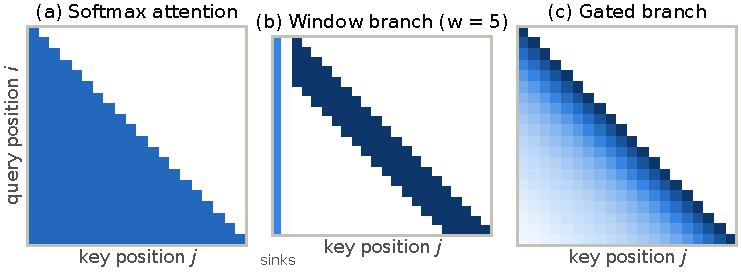
\includegraphics[width=\linewidth]{attention_patterns}
\caption[Keys that each type of attention uses]{Keys that each type of attention uses, in a toy example with 20 positions. Each row is a query and each column is a key. Darker cells have more weight. (a)~Softmax attention can use every earlier key. (b)~The window branch uses only the last $w$ keys, plus the sink logits on the left. (c)~The gated branch uses every earlier key, but the gate makes the weight smaller with the distance. Panel (c) uses a constant gate of 0.82.}
\label{fig:patterns}
\end{figure}

\section{Knowledge distillation and attention transfer}
\label{sec:distill}

In knowledge distillation~\cite{hinton2015}, a student model learns from the outputs of a teacher model. Linearization uses a special form: the student and the teacher have the same weights, except for the attention. Thus each student attention layer can learn directly from the teacher attention layer. The loss compares the two outputs of each layer with the mean squared error (MSE). This is \emph{attention transfer}. Each student layer gets the input of the teacher layer, not the output of the student layer before it. Thus an error in one layer does not change the input of the next layer during this training.

\section{Low-rank adaptation}
\label{sec:lora}

Attention transfer trains each layer alone. The full model can still lose quality. A second stage trains the whole model with the next-token loss. LoRA~\cite{lora} makes this stage cheap. It keeps a weight matrix $W$ frozen and adds a product of two small matrices: $W + \frac{\alpha_{\text{LoRA}}}{r} BA$, with the rank $r$. In this work, $r = 8$ and $\alpha_{\text{LoRA}} = 16$. With LoRA on the four attention projections, stage 2 trains 1,703,936 parameters, which is approximately 0.14\% of the model.

\section{How the harness scores multiple-choice tasks}
\label{sec:scoring}

The evaluation of this thesis does not let the model write an answer. For each question, the harness builds one text for each answer option. It computes the log-likelihood of the option after the question. The option with the highest value counts as the answer of the model. The metric \code{acc} uses the raw log-likelihood. The metric \code{acc_norm} divides it by the length of the option text, so that long options are not at a disadvantage.

MMLU uses a different format. The prompt lists four options with the letters A to D and ends with \enquote{Answer:}. The harness compares the log-likelihoods of the four tokens \enquote{ A} to \enquote{ D}. The model must therefore connect its knowledge with the right letter. PIQA and ARC use the full text of each option, so a preference for one letter has no effect there.

\section{The benchmarks}
\label{sec:benchmarks}

\Cref{tab:benchmarks} lists the benchmarks of this thesis. The paper of Lizard uses the same six benchmarks in its Table~9.

\begin{table}[ht]
\centering
\small
\caption[The benchmarks of this thesis]{The benchmarks of this thesis. All tasks are multiple choice. MMLU uses 5 examples before each question (5-shot). The other tasks use no examples (0-shot).}
\label{tab:benchmarks}
\begin{tabularx}{\linewidth}{@{}lLrcc@{}}
\toprule
Benchmark & Content & Questions & Options & Metric of the paper \\
\midrule
MMLU~\cite{mmlu} & Knowledge in 57 subjects, from high school to professional level & 14,042 & 4 & \code{acc}, 5-shot \\
PIQA~\cite{piqa} & Physical commonsense: a goal and two solutions & 1,838 & 2 & \code{acc} \\
ARC-Easy~\cite{arc} & Grade-school science questions, Easy set & 2,376 & 4 & \code{acc} \\
ARC-Challenge~\cite{arc} & Grade-school science questions, Challenge set & 1,172 & 4 & \code{acc_norm} \\
HellaSwag~\cite{hellaswag} & The most probable end of a short story & 10,042 & 4 & \code{acc_norm} \\
WinoGrande~\cite{winogrande} & Pronoun resolution in a sentence & 1,267 & 2 & \code{acc} \\
\bottomrule
\end{tabularx}
\end{table}

The chance level is 25\% for four options and 50\% for two options. The teacher is a small model, and it gets only 31.0 on MMLU in the paper. Thus the MMLU scores of all 1B models lie close to chance, and small differences need many questions. Appendix~\ref{app:definitions} gives short definitions of further terms, such as packing and padding.

% Chapter 3
\chapter{Related Work}
\label{ch:related}

\section{Linear attention and recurrent models}
\label{sec:rw-linear}

Katharopoulos et al.~\cite{katharopoulos2020} showed that linear attention is a recurrent network with a matrix state. Later work added gates and better feature maps. GLA~\cite{gla} uses a gate for each key dimension and trains models from the start. Mamba-2~\cite{mamba2} connects state space models with linear attention. Based~\cite{based} joins linear attention with a small sliding window. The window gives exact local attention, and the linear part gives the long range. Lizard uses the same idea. These models need a full pretraining run. Linearization avoids this cost.

\section{Linearization methods: LoLCATs, Liger and Lizard}
\label{sec:rw-linearization}

\textbf{LoLCATs}~\cite{lolcats} trains Hedgehog feature maps to copy the attention of a teacher (attention transfer), then trains LoRA weights. Its window has RoPE, and its linear part covers only the tokens before the window. The window and the linear part share one denominator. On Llama-3-8B, LoLCATs with 50\% softmax layers gets 65.8 on MMLU, against 52.8 for the fully linear model and 66.6 for the teacher.

\textbf{Liger}~\cite{liger} has no attention transfer stage and adds no new parameters. It uses the teacher projections in a GLA form with a fixed feature map. It mixes a gated branch and a window with the factor 0.5 each. The paper writes the window without RoPE, but the code of Liger applies RoPE. Liger trains only LoRA weights with the next-token loss.

\textbf{Lizard}~\cite{lizard} keeps the attention transfer stage of LoLCATs. It adds a learned scalar gate, four sink logits and the weight $\alpha$. Its window has no RoPE by design. The paper wants the gate to learn the relative position, so that the model can work on inputs longer than in training. \Cref{tab:methods} compares the three methods with GLA. \Cref{sec:fourmethods} gives the formulas.

\begin{table}[ht]
\centering
\small
\caption[Four attention methods side by side]{Four attention methods side by side. The values come from the papers and the code of each method (project notes, document~15).}
\label{tab:methods}
\begin{tabularx}{\linewidth}{@{}lLLLL@{}}
\toprule
Part & Lizard & LoLCATs & Liger & GLA \\
\midrule
Feature map & Hedgehog, learned, shared by the heads & Hedgehog, learned, one for each head & Softmax over the head dimension, no weights & None \\
Gate & One scalar for each token & None & From the key, power 1/16 (code) & One value for each key dimension \\
Window & 128 keys, 4 sinks, no RoPE & 64 keys, RoPE & 64 keys, RoPE in the code & None \\
Tokens in the linear part & All earlier tokens & Only tokens before the window & All earlier tokens & All earlier tokens \\
Denominator & Own row sum for each branch & Shared by both parts & None in the linear part & None \\
Total weight of a row & $1 + \alpha\rho_i$ & 1 & $0.5 + 0.5\mu_i$ & -- \\
Training & Attention transfer, then LoRA & Attention transfer, then LoRA & LoRA only & Pretraining \\
\bottomrule
\end{tabularx}
\end{table}

\section{Linearized models at the 1B scale}
\label{sec:rw-1b}

Other papers also report weak MMLU scores for linearized 1B models. \Cref{tab:rw-1b} collects the numbers that the project notes found. The Liger paper reports 23.1 for LoLCATs and 22.4 for Liger on Llama-3.2-1B. The Lizard paper reports 27.3 for LoLCATs on the same model. Thus two papers give different values for the same method, and the evaluation details matter. STILL~\cite{still} keeps exact softmax attention over selected tokens and reports 29.8.

\begin{table}[ht]
\centering
\small
\caption[Reported results of linearized Llama-3.2-1B models]{Reported results of linearized Llama-3.2-1B models. Each paper uses its own harness. The values are accuracies in \%.}
\label{tab:rw-1b}
\begin{tabular}{@{}llrrr@{}}
\toprule
Source & Model & MMLU & PIQA & ARC-Easy \\
\midrule
Lizard paper, Table 9 & Teacher & 31.0 & 74.1 & 65.4 \\
 & LoLCATs & 27.3 & 74.6 & 63.0 \\
 & Lizard & 29.8 & 74.8 & 65.6 \\
Liger paper, Table 4 & Teacher & 31.0 & -- & -- \\
 & LoLCATs & 23.1 & 74.1 & 63.7 \\
 & Liger & 22.4 & 75.0 & 65.4 \\
STILL & STILL & 29.8 & -- & -- \\
\bottomrule
\end{tabular}
\end{table}

Two more results connect to this thesis. RADLADS~\cite{radlads} uses a second stage with the Kullback--Leibler (KL) divergence to the teacher logits, not the next-token loss on new data. A report with the title \enquote{Stuck on A}~\cite{stuckona} describes a linearized 0.6B model with a perplexity near the teacher. But the model has chance accuracy on multiple-choice tasks, and it gives the answer \enquote{A} for 81\% of the questions. \Cref{ch:repro} describes the same symptom.

\section{Hybrid models and retrieval heads}
\label{sec:rw-hybrid}

Several methods keep a small part of the softmax attention. Bick et al.~\cite{bick2025} study \emph{gather-and-aggregate} (G\&A) heads. A few such heads do the letter step of MMLU. In a pruned Llama-3.1-8B, one disabled G\&A head drops MMLU from 66\% to 25\%. Recurrent models give smoother attention patterns, without the sharp attention that these heads need. DuoAttention~\cite{duoattention} keeps full attention for a few retrieval heads and uses a window with sinks for the other heads. A KL-guided method~\cite{klselect} selects which layers stay softmax. LoLA~\cite{lola} adds a small cache of tokens that linear attention cannot recall. These ideas are options for the MMLU gap (\cref{ch:conclusion}).

\section{Interpretability of distilled attention}
\label{sec:rw-xai}

The LoLCATs paper plots the error of each layer after attention transfer (its Figure~14). It also compares the attention weights of the teacher and the student (its Figures~18--21). \Cref{ch:xai} uses both methods. Further methods exist, for example activation patching~\cite{heimersheim2024}, induction heads~\cite{olsson2022} and the tuned lens~\cite{belrose2023}. This thesis does not use them, but \cref{ch:conclusion} lists them as next steps.

% Chapter 4
\chapter{Lizard and Its Implementation}
\label{ch:lizard}

\section{Lizard attention}
\label{sec:lizard-attn}

Lizard~\cite{lizard} replaces every softmax attention layer of the teacher with two branches (\cref{fig:lizard-layer}). The teacher projections $W_Q$, $W_K$, $W_V$ and $W_O$ stay as they are. Lizard adds five small parameters to each layer.

\begin{description}[leftmargin=0.6cm,style=nextline]
\item[Gated branch] Gated linear attention (\cref{eq:gla}) with Hedgehog feature maps $\phi_q$ and $\phi_k$ (\cref{eq:hedgehog}). The gate is one scalar for each token, $\gamma_i = \sigma(W_\gamma \vx_i)$. All 32 heads of a layer share the feature maps and the gate. The branch divides by its own row sum, so its weights sum to 1.
\item[Window branch] Softmax attention over the last $w = 128$ keys, with $m = 4$ sink logits in the denominator (\cref{eq:window}). The paper calls it \emph{anchor window attention}. It has no RoPE.
\item[Output] The two branches add up: $\hat\vy_i = \hat\vy^{\text{gate}}_i + \alpha\, \hat\vy^{\text{win}}_i$, with one learnable $\alpha$ for each layer.
\end{description}

\begin{figure}[t]
\centering
\resizebox{\linewidth}{!}{%
\begin{tikzpicture}[
  font=\small, >={Stealth[length=2.2mm]}, node distance=6mm,
  box/.style={draw=#1, fill=#1!10, rounded corners=1.5pt, align=center, inner sep=4pt, line width=0.6pt},
  teacher/.style={box=teachercolor, text width=3.4cm},
  lizard/.style={box=lizardcolor, text width=3.9cm},
  small/.style={box=lizardcolor, text width=1.6cm},
  opt/.style={draw=changecolor, fill=changecolor!8, dashed, rounded corners=1.5pt, align=center, inner sep=4pt, text width=3.9cm, line width=0.6pt},
  arr/.style={->, draw=inksecondary, line width=0.6pt}]
\node[box=teachercolor, text width=1.6cm] (x) at (0,0) {input $\vx_i$};
\node[teacher] (proj) at (0,-1.35) {$W_Q,\ W_K,\ W_V$\\ \footnotesize teacher weights};
\node[small, text width=1.7cm] (gate) at (-6.8,-3.0) {gate $W_\gamma$\\[1pt] \footnotesize $\sigma(W_\gamma \vx_i)$};
\node[lizard] (phi) at (-3.6,-3.0) {Hedgehog maps $\phi_q,\ \phi_k$\\ \footnotesize shared by the 32 heads};
\node[opt] (rope) at (3.6,-3.0) {RoPE on $\vq,\ \vk$\\ \footnotesize only in \code{window_rope}};
\node[lizard] (gla) at (-3.6,-4.85) {\textbf{Gated branch}\\ \footnotesize all keys $t \le i$, weight $\prod_{l=t+1}^{i}\gamma_l$, own row sum};
\node[lizard] (win) at (3.6,-4.85) {\textbf{Window branch}\\ \footnotesize softmax over the last 128 keys};
\node[small] (sink) at (6.6,-4.85) {sinks\\ $t_1, \dots, t_4$};
\node[circle, draw=lizardcolor, fill=lizardcolor!10, inner sep=1.5pt, line width=0.6pt] (alpha) at (3.6,-6.35) {$\times\,\alpha$};
\node[circle, draw=inksecondary, inner sep=1pt, line width=0.6pt] (plus) at (0,-7.05) {$+$};
\node[teacher] (oproj) at (0,-8.1) {$W_O$\\ \footnotesize teacher weight};
\node[box=teachercolor, text width=1.6cm] (y) at (0,-9.25) {output};
\draw[arr] (x) -- (proj);
\draw[arr] (x.west) -| (gate.north);
\draw[arr] (proj.south) -- ++(0,-0.4) -| (phi.north);
\draw[arr] (proj.south) -- ++(0,-0.4) -| (rope.north);
\draw[arr] (phi) -- (gla);
\draw[arr] (rope) -- (win);
\draw[arr] (gate.south) |- node[pos=0.75, above, font=\footnotesize, text=inksecondary] {$\gamma_i$} (gla.west);
\draw[arr] (sink) -- (win);
\draw[arr] (proj.south) -- node[right, font=\footnotesize, text=inksecondary, pos=0.6] {$\vv$} (0,-4.85) -- (gla.east);
\draw[arr] (0,-4.85) -- (win.west);
\draw[arr] (win) -- (alpha);
\draw[arr] (alpha) |- (plus);
\draw[arr] (gla) |- (plus);
\draw[arr] (plus) -- (oproj);
\draw[arr] (oproj) -- (y);
\node[box=lizardcolor, minimum width=4mm, minimum height=3mm, inner sep=0pt] (l1) at (-6.4,-8.65) {};
\node[right=1mm of l1, font=\footnotesize, align=left] {Lizard parameters,\\trained in stage 1};
\node[box=teachercolor, minimum width=4mm, minimum height=3mm, inner sep=0pt] (l2) at (-6.4,-9.45) {};
\node[right=1mm of l2, font=\footnotesize, align=left] {teacher weights,\\LoRA in stage 2};
\end{tikzpicture}%
}
\caption[One Lizard attention layer]{One Lizard attention layer. The teacher projections give the queries $\vq$, the keys $\vk$ and the values $\vv$. Blue parts are the Lizard parameters. Gray parts are the weights of the teacher. The purple RoPE box is the change of \cref{ch:rope}. The original Lizard has no RoPE in either branch.}
\label{fig:lizard-layer}
\end{figure}

\Cref{tab:lizard-params} lists the parameters of one layer. Lizard adds 18,437 parameters to each layer and 294,992 to the 16 layers. This is 0.024\% of the model.

\begin{table}[ht]
\centering
\small
\caption[The Lizard parameters of one layer]{The Lizard parameters of one layer, with feature dimension 128 (project notes, document~1).}
\label{tab:lizard-params}
\begin{tabularx}{\linewidth}{@{}llrL@{}}
\toprule
Parameter & Shape & Count & Function \\
\midrule
\code{phi_q}, \code{phi_k} & $64 \times 128$ each & 16,384 & Feature maps with 256 features. All heads share them. \\
\code{W_gamma} & $2048 \times 1$ & 2,048 & Gate. Start value 0, so $\gamma = 0.5$ at the start. \\
\code{meta_tokens} & 4 & 4 & Sink logits in the window denominator \\
\code{alpha_blend} & 1 & 1 & Weight $\alpha$ of the window branch. Start value 1. \\
\midrule
Total & & 18,437 & \\
\bottomrule
\end{tabularx}
\end{table}

\section{The two training stages}
\label{sec:stages}

\Cref{fig:stages} shows the two stages as the paper describes them.

\textbf{Stage 1: attention transfer.} Only the Lizard parameters train. Each Lizard layer gets the input of the teacher layer. The teacher computes its own output with RoPE. The loss compares the two outputs of each layer:
\begin{equation}
\mathcal{L}_{\text{MSE}} = \frac{1}{N} \sum_{l=1}^{N} \left\| \mathbf{Y}^{l}_{\text{softmax}} - \hat{\mathbf{Y}}^{l}_{\text{Lizard}} \right\|_F^2 .
\label{eq:stage1}
\end{equation}
The code of this work uses 1000 times the mean squared error of each layer. This form differs from \cref{eq:stage1} only by a constant factor, and the Adam optimizer does not change with such a factor.

\textbf{Stage 2: fine-tuning.} LoRA weights on the attention projections train with the next-token loss. In the code of this work, the Lizard parameters stay frozen in stage 2. The paper does not say if they train.

\begin{figure}[t]
\centering
\begin{subfigure}{0.82\linewidth}
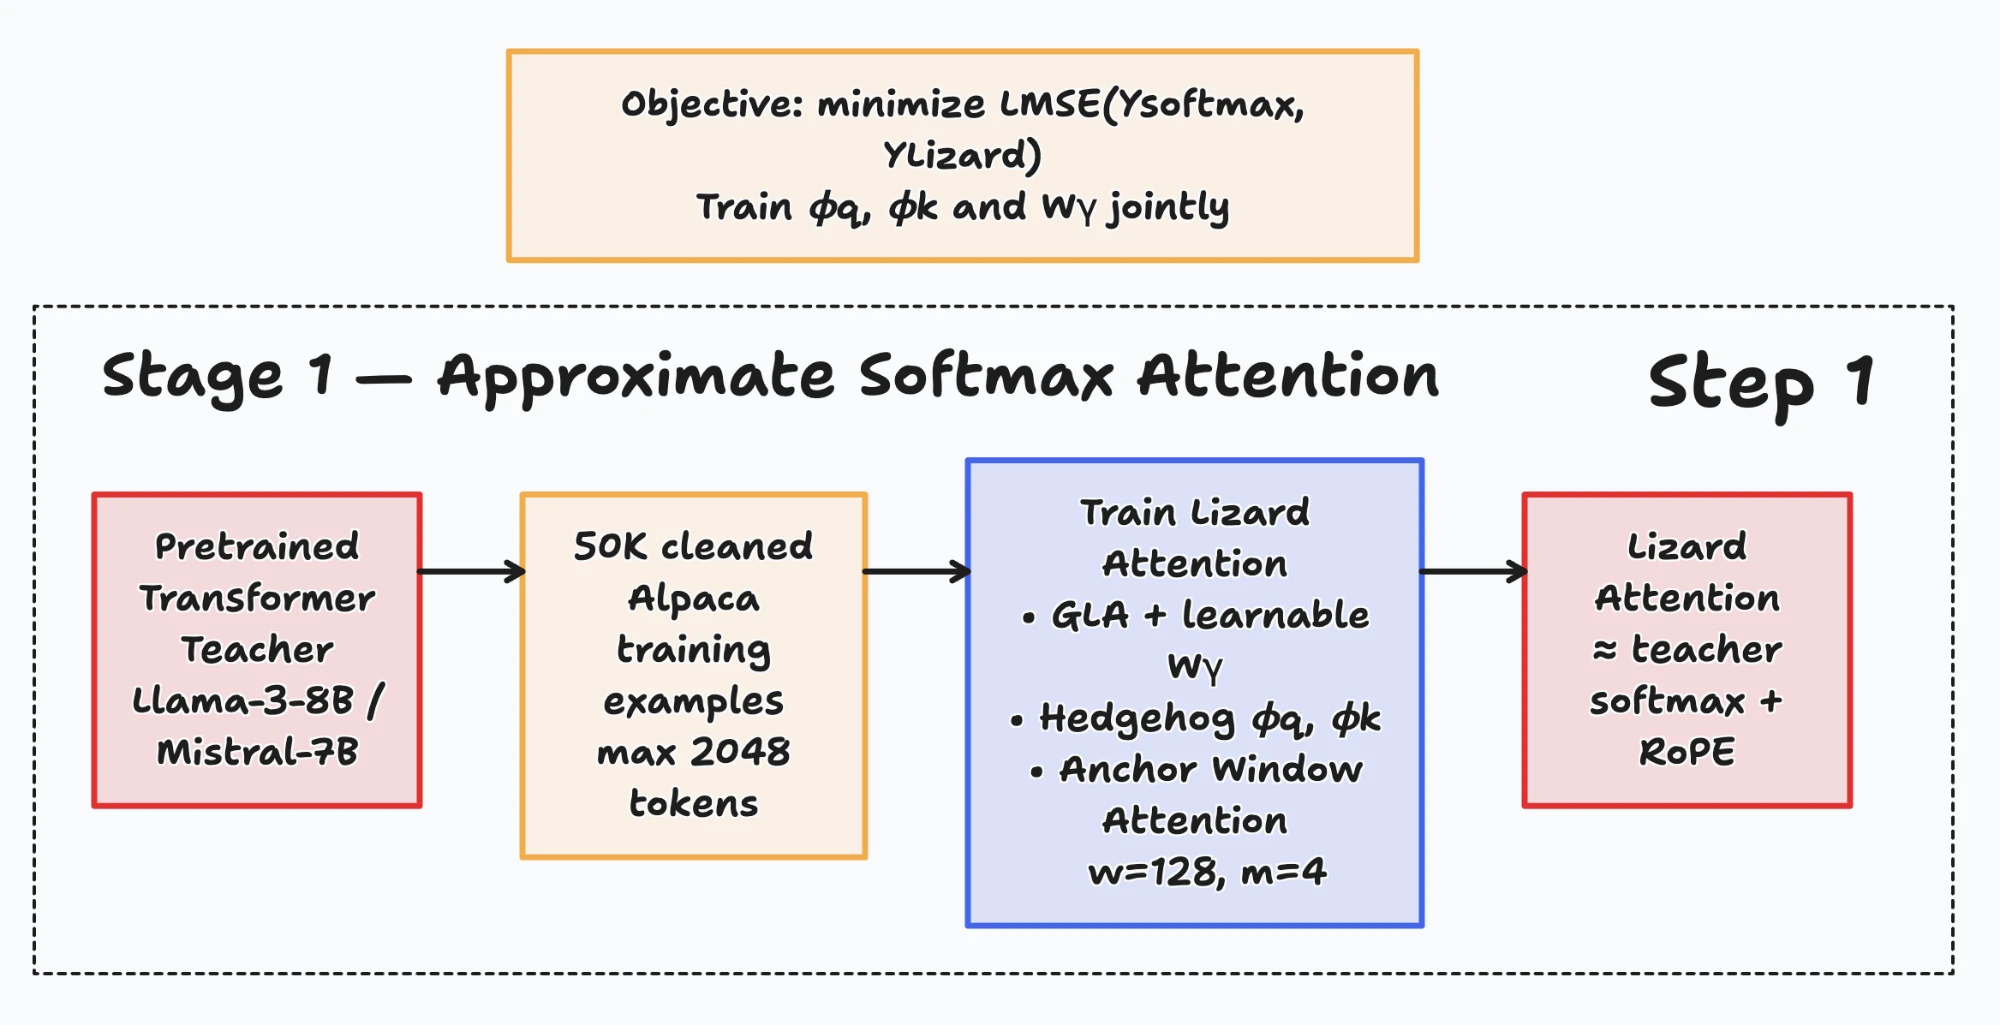
\includegraphics[width=\linewidth]{lizard-stage1}
\caption{Stage 1: attention transfer with the MSE loss.}
\end{subfigure}\\[6pt]
\begin{subfigure}{0.82\linewidth}
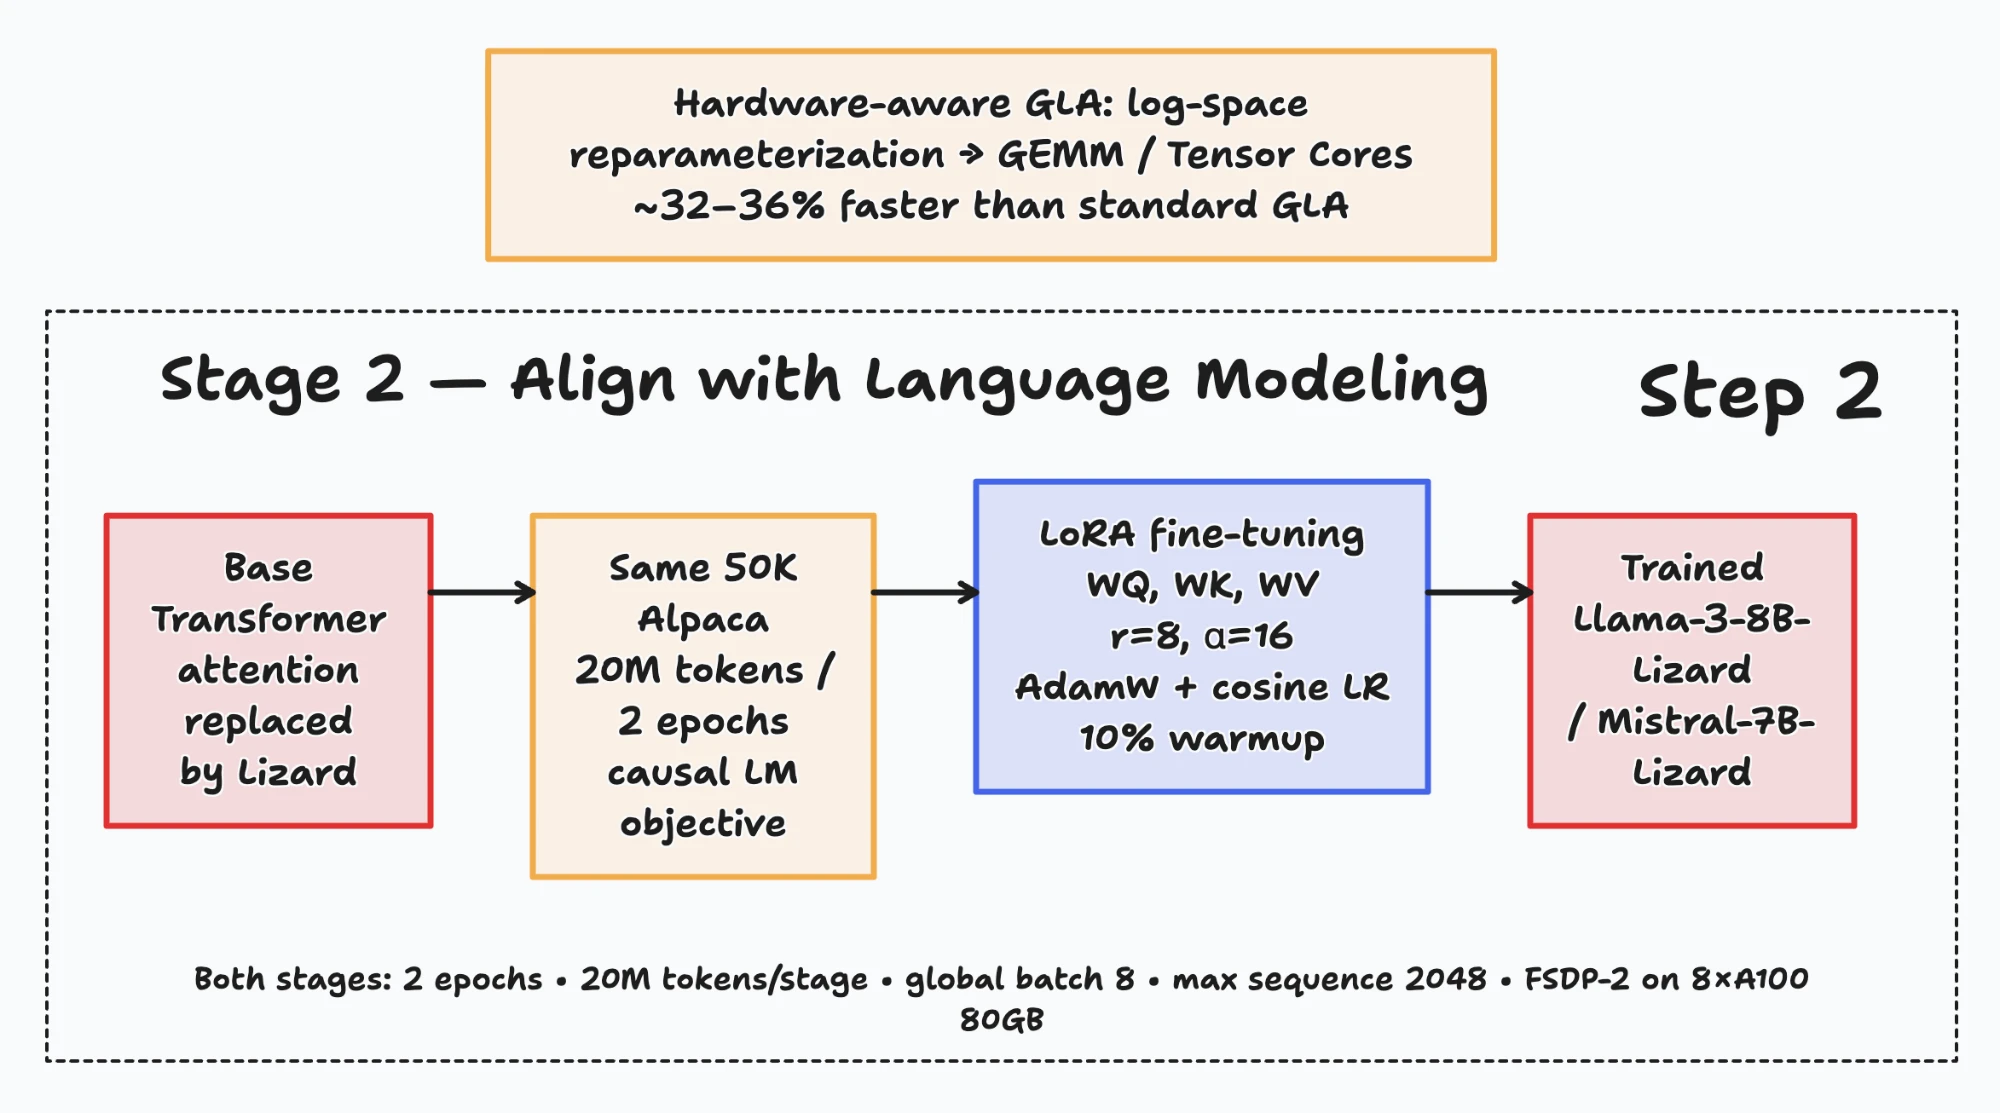
\includegraphics[width=\linewidth]{lizard-stage2}
\caption{Stage 2: LoRA with the next-token loss.}
\end{subfigure}
\caption[The two training stages of Lizard]{The two training stages of Lizard, as the paper describes them. The paper uses 8B teachers in this description. This thesis uses Llama-3.2-1B. Source: the figures of the project notes, drawn by the author.}
\label{fig:stages}
\end{figure}

\section{The training algorithm in log space}
\label{sec:logspace}

Section~4 of the paper gives a fast algorithm for the gated branch. In matrix form, the branch needs the cumulative gate products $c_t = \prod_{j \le t} \gamma_j$ and the quotients $c_i / c_t$. The products get very small, and bf16 cannot store them. The paper moves $\log c_t$ into the exponent of the feature maps, so that the branch becomes one matrix product.

A proof audit of this work found a limit (\cref{tab:proofs}, P3). The step holds for the exponential feature map. With the softmax feature map of Table~13, the term $\log c_t$ cancels in the softmax, and the gate disappears. Also, $1/c_t$ overflows after approximately 126 tokens at $\gamma = 0.5$, so only a form that works in chunks can use it. This work does not use the fast algorithm. It computes the parallel form of \cref{eq:gla} in float32 and materializes the full $L \times L$ matrix.

\section{The reference implementation}
\label{sec:reference}

The work started with a reference implementation in the repository \code{jku-thesis}~\cite{jkurepo}. It is pure PyTorch. The functions \code{hedgehog}, \code{gla} and \code{awa} implement the formulas directly, and a class \code{LizardAttention} joins them. A second file contains slow loop and recurrent versions of every formula. These versions are the ground truth. The tests compare the two versions in float64 and require a relative error below $10^{-10}$. Further adapters compare the branches with external implementations, for example the GLA kernels of the \code{flash-linear-attention} library and PyTorch attention with a sink column.

\section{The port to LoLCATs}
\label{sec:port}

The training of this work uses the LoLCATs code base~\cite{lolcats,lolcatsrepo}. It already has the two stages, the data pipeline and the evaluation. The functions of the reference code went into LoLCATs without changes. A wrapper class connects them with the LoLCATs model:

\begin{itemize}
\item It takes the teacher attention module and uses its projections again. Thus only the five Lizard parameters are new.
\item In stage 1, it computes the teacher output with RoPE as the target. It returns the student output and the target to the trainer. The next layer gets the teacher output.
\item In evaluation and generation, it uses a cache. The cache keeps the state of the gated branch and the keys and values of the last 128 tokens. A prompt runs in one dense pass. Each new token then uses the recurrent form.
\end{itemize}

\Cref{tab:jku-vs-lolcats} shows the differences between the two code bases. The LoLCATs recipe became the first recipe of this work, because the task was to keep the existing configs.

\begin{table}[ht]
\centering
\small
\caption[The reference pipeline against the LoLCATs pipeline]{The reference pipeline (\code{jku-thesis}) against the LoLCATs pipeline of the first runs (project notes, document~1).}
\label{tab:jku-vs-lolcats}
\begin{tabularx}{\linewidth}{@{}lLL@{}}
\toprule
Aspect & Reference pipeline & LoLCATs pipeline \\
\midrule
Stage 1 loss & Summed squared error for each layer & 1000 $\times$ mean squared error for each layer \\
Stage 2 parameters & LoRA on $q, k, v$ and the Lizard parameters & LoRA on $q, k, v, o$. Lizard parameters frozen. \\
Precision & float32 & bf16 model, Lizard computations in float32 \\
Recipe & The recipe of the paper & The LoLCATs configs: learning rate $10^{-2}$ in stage 1 and $10^{-4}$ in stage 2 \\
\bottomrule
\end{tabularx}
\end{table}

\section{Tests of the attention layer}
\label{sec:tests}

The poor first results (\cref{ch:repro}) raised the question of a bug. Two levels of tests ran on CPU.

\textbf{Level 1: the formulas.} A small module made the 28 tests of the reference code run against the LoLCATs functions. 26 tests passed. The two other tests need a newer version of the \code{transformers} library and fail for the same reason on the reference code. The tests show these properties: the feature maps are positive, and each half sums to 1. The gated branch matches the loop form and the recurrent form. The window with sinks matches its loop form. Future tokens give no gradient. The gradients match finite differences.

\textbf{Level 2: the model.} A tiny Llama with random weights in float64 tested the wrapper, the conversion of the model and the cached paths. The output with the cache equals the dense output up to float64 rounding.

\begin{finding}
The tests show that the code computes the equations of the paper, and that the evaluation path computes the same function as the training path. They do not test the quality of the trained weights.
\end{finding}

\section{The paper against the code}
\label{sec:paper-vs-code}

A line-by-line comparison of the formulas of the paper with the code found 17 differences. Most of them have no effect. \Cref{tab:open-points} lists the points where the paper allows more than one reading.

\begin{table}[ht]
\centering
\small
\caption[Open points of the paper]{Open points of the paper and the choice of the code (project notes, documents~9, 13 and \enquote{math against code}).}
\label{tab:open-points}
\begin{tabularx}{\linewidth}{@{}>{\raggedright\arraybackslash}p{3.3cm}LL@{}}
\toprule
Point & What the paper says & Choice of the code \\
\midrule
D1: normalization of the gated branch & The parallel form has a denominator. The recurrent form and the matrix form have none. & Denominator (row sum 1) \\
D2: feature maps for each head & Not given. The LoLCATs default has one map for each head. & One map for all heads of a layer \\
D3: activation & Section 4 gives $\exp$. Table 13 gives softmax. & Softmax \\
D5: sink term & The equation has $\sum_j t_j$, but the text calls $t_j$ a logit. & $\sum_j \exp(t_j)$ \\
Gate start value & Not given & $W_\gamma = 0$, so $\gamma = 0.5$ \\
$\alpha$ & Not listed as a learnable parameter in the loss & Learnable, start value 1 \\
\bottomrule
\end{tabularx}
\end{table}

The written sink term $\sum_j t_j$ can make the denominator zero or negative (\cref{tab:proofs}, P4). Thus the code follows the word \enquote{logit}.

\section{Lizard attention v2: one option for each reading}
\label{sec:v2}

A second attention file (v2) makes each open point an option. With the default options, v2 gives exactly the outputs of v1. \Cref{tab:v2-options} lists the options.

\begin{table}[ht]
\centering
\small
\caption[The options of Lizard attention v2]{The options of Lizard attention v2. The first value is the default (project notes, document~13).}
\label{tab:v2-options}
\begin{tabularx}{\linewidth}{@{}lp{3.3cm}L@{}}
\toprule
Option & Values & Meaning \\
\midrule
\code{gla_norm} & \code{row}, \code{none}, \code{joint}, \code{hybrid} & Row sum of the gated branch (D1). \code{joint} and \code{hybrid} use one denominator for both branches and the sinks. \code{hybrid} is the LoLCATs form. \\
\code{alpha_per_head} & false, true & One $\alpha$ for each head \\
\code{alpha_init} & 1.0, any number & Start value of $\alpha$ \\
\code{feature_map_per_head} & false, true & One feature map for each head (D2) \\
\code{feature_activation} & softmax, exp & D3 \\
\code{gate_per_head} & false, true & One gate for each head \\
\code{gate_bias_init} & none, a number & A bias in the gate with a start value \\
\code{window_rope} & false, true & RoPE in the window branch only \\
\bottomrule
\end{tabularx}
\end{table}

\section{Proofs and float64 tests}
\label{sec:proofs}

The options depend on claims about the formulas. A proof audit checked each claim by hand. A float64 script then computed the smallest cases. \Cref{tab:proofs} lists the main claims.

\begin{table}[ht]
\centering
\small
\caption[Main claims of the proof audits]{Main claims of the proof audits (project notes, documents~13, 14 and 15). \enquote{Restricted} means: true only under the stated condition.}
\label{tab:proofs}
\begin{tabularx}{\linewidth}{@{}lLl@{}}
\toprule
Claim & Statement & Verdict \\
\midrule
P1 & The recurrent form equals the parallel form, without and with the denominator & Proved \\
P2 & The window share of a head is at most $\alpha / (1 + \alpha)$ & Restricted: $\alpha \ge 0$ \\
P3 & The log-space form equals the gated matrix form & Only for the $\exp$ map \\
P4 & The written sink term $\sum_j t_j$ can make the denominator 0 or negative & Proved \\
P5 & The decode forms of \code{joint} and \code{window_rope} equal their parallel forms & Proved \\
P6 & \code{joint} keeps a usable share for the gated branch at the start & Refuted \\
P7 (H) & Four sink logits with equal start values stay equal, so they act as one sink & Proved \\
P8 (C) & The total weight of a Lizard row is $1 + \alpha\rho_i$, more than 1 & Proved \\
P9 & With \code{hybrid} and $\gamma = 1$, the window share falls as $1/i$ & Restricted \\
P10 (F) & A window without RoPE cannot give exact previous-token attention in layer 0 & Restricted: no position input \\
\bottomrule
\end{tabularx}
\end{table}

Three claims matter most for the later chapters. P8 shows that a Lizard row is not a weighted mean of values: its weights sum to more than 1. P2 shows that $\alpha$ limits how much a head can take from the exact window. P10 shows that the window without RoPE cannot find the previous token from the positions.

\section{Lizard, LoLCATs, GLA and Liger in formulas}
\label{sec:fourmethods}

With the notation $\kappa_{it} = \phi(\vq_i)^\top\phi(\vk_t)$, the gate products $c_{it}$ and the window scores $s_{it}$, the outputs of Lizard and LoLCATs are
\begin{align}
\text{Lizard:}\quad \vy_i &= \frac{\sum_{t \le i} c_{it}\, \kappa_{it}\, \vv_t}{\sum_{t \le i} c_{it}\, \kappa_{it}} + \alpha\, \frac{\sum_{t \in W_i} e^{s_{it}} \vv_t}{\sum_{j} e^{t_j} + \sum_{t \in W_i} e^{s_{it}}}, \\
\text{LoLCATs:}\quad \vy_i &= \frac{\sum_{t \in W_i} a\, e^{s_{it}} \vv_t + \sum_{t \le i - w} \kappa_{it}\, \vv_t}{\sum_{t \in W_i} a\, e^{s_{it}} + \sum_{t \le i - w} \kappa_{it}} .
\end{align}
LoLCATs gives an exact weighted mean of the values. Its linear part excludes the window tokens. Lizard counts the window tokens twice, one time in each branch (claim B of document~15). The \code{hybrid} option of v2 equals LoLCATs under three conditions (claim A). All gates are 1, there are no sinks, and the linear sums cover only $t \le i - w$.

\section{Numerical stability: the NaN crash}
\label{sec:nan}

The first full run stopped in stage 2 at gradient step 386. The forward pass gave NaN, and a debugger breakpoint in the trainer then ended the job. A review found two operations without protection:

\begin{itemize}
\item The window branch computed $\exp(\vq^\top\vk/\sqrt{d})$ directly. In float32, $\exp$ overflows above approximately 88.7, and $\infty/\infty$ gives NaN. LoRA trains the query and key projections in stage 2, so the scores can grow.
\item The gated branch divides by the row sum. If all weights of a row underflow to 0, the result is $0/0$.
\end{itemize}

The fix subtracts the largest score and the largest sink logit before $\exp$, and it gives the row sum a small lower limit. Both changes keep the formulas the same. The overflow is the most probable cause, but no test reproduced it on the real checkpoint.

% Chapter 5
\chapter{Experimental Setup}
\label{ch:setup}

\section{The teacher and the data}
\label{sec:data}

The teacher is \code{meta-llama/Llama-3.2-1B} in bf16, with the model sizes of \cref{sec:softmax}. Both stages use the cleaned Alpaca data set~\cite{alpaca} (\code{yahma/alpaca-cleaned}), as the paper does. The pipeline joins the examples and cuts the text into sequences of 2048 tokens. This is \emph{packing} (Appendix~\ref{app:definitions}). \Cref{tab:data} gives the sizes.

\begin{table}[ht]
\centering
\small
\caption[Data of both training stages]{Data of both training stages (measured in the first run, project notes, document~2).}
\label{tab:data}
\begin{tabular}{@{}lr@{}}
\toprule
Quantity & Value \\
\midrule
Training examples & 51,560 \\
Validation examples & 200 \\
Sequences of 2048 tokens in each epoch & 4,714 (approximately 9.7 million tokens) \\
Epochs in each stage & 2 \\
Sequences in each gradient step & 8 (batch 1 $\times$ 8 accumulation steps) \\
Gradient steps in each stage & 1,178 \\
Validation & every 100 steps \\
\bottomrule
\end{tabular}
\end{table}

\section{The training recipes}
\label{sec:recipes}

The first runs used the existing LoLCATs configs. Their recipe differs from the recipe of the paper in several points (\cref{tab:recipes}). The most important differences are the learning rate of stage 1, the schedule and the gradient clipping. \Cref{ch:gap} tests these differences one at a time.

\begin{table}[ht]
\centering
\small
\caption[The LoLCATs recipe against the recipe of the paper]{The LoLCATs recipe of the first runs against the recipe of the paper. Sources: Section 5 and Table 13 of the paper, project notes, documents~4 and 9. Bold rows are the largest differences.}
\label{tab:recipes}
\begin{tabularx}{\linewidth}{@{}lLL@{}}
\toprule
Setting & Paper & First runs (LoLCATs configs) \\
\midrule
Data & Alpaca-cleaned, 2 epochs, 2048 tokens & The same \\
Global batch & 8 (micro batch 1) & The same \\
Precision & bf16 & bf16 model, Lizard computations in float32 \\
\textbf{Learning rate, stage 1} & $\mathbf{10^{-3}}$ & $\mathbf{10^{-2}}$ \textbf{(10$\times$ higher)} \\
Learning rate, stage 2 & $5 \times 10^{-4}$ & $10^{-4}$ (5$\times$ lower) \\
\textbf{Schedule} & \textbf{Cosine, 10\% warmup, minimum 0.1$\times$ peak} & \textbf{Almost constant (reduce on plateau), no warmup} \\
\textbf{Gradient clipping} & \textbf{1.0} & \textbf{None} \\
AdamW $\beta$ & (0.9, 0.99) & (0.9, 0.999) \\
LoRA & $r = 8$, $\alpha = 16$, on $W_Q, W_K, W_V$ & $r = 8$, $\alpha = 16$, on $q, k, v$ and $o$ \\
Lizard parameters in stage 2 & Not given & Frozen \\
Checkpoint & Not given & Best validation loss \\
\bottomrule
\end{tabularx}
\end{table}

\section{Infrastructure}
\label{sec:infra}

\Cref{fig:pipeline} shows the path from a code change to a result. A GitHub workflow builds a Docker image with the training code. Hugging Face Jobs runs the image on one rented GPU. The job pushes the checkpoints to a private model repository on the Hugging Face Hub. A university machine with one NVIDIA A10 (24~GB) then downloads the checkpoints and runs the evaluation. W\&B logs the training curves.

\begin{figure}[ht]
\centering
\resizebox{\linewidth}{!}{%
\begin{tikzpicture}[font=\small, >={Stealth[length=2mm]},
  pbox/.style={draw=lizardcolor, fill=lizardcolor!8, rounded corners=1.5pt, align=center, text width=2.4cm, minimum height=1.55cm, inner sep=3pt, line width=0.6pt},
  arr/.style={->, draw=inksecondary, line width=0.6pt}]
\node[pbox] (git) at (0,0) {\textbf{GitHub}\\ \footnotesize code, configs,\\ pull requests};
\node[pbox] (img) at (3.3,0) {\textbf{GitHub Actions}\\ \footnotesize builds the\\ Docker image};
\node[pbox] (job) at (6.6,0) {\textbf{HF Jobs}\\ \footnotesize one H200:\\ stage 1, stage 2};
\node[pbox] (hub) at (9.9,0) {\textbf{HF Hub}\\ \footnotesize private\\ checkpoints};
\node[pbox] (eval) at (9.9,-2.9) {\textbf{University A10}\\ \footnotesize evaluation and\\ XAI scripts};
\node[pbox] (docs) at (6.6,-2.9) {\textbf{Project notes}\\ \footnotesize results, plots,\\ decisions};
\node[pbox, draw=teachercolor, fill=teachercolor!8] (wandb) at (3.3,-2.9) {\textbf{W\&B}\\ \footnotesize training curves};
\draw[arr] (git) -- (img);
\draw[arr] (img) -- (job);
\draw[arr] (job) -- (hub);
\draw[arr] (hub) -- (eval);
\draw[arr] (eval) -- (docs);
\draw[arr] (job.south) -- ++(0,-0.55) -| (wandb.north);
\draw[arr] (docs.south) -- ++(0,-0.35) -| node[pos=0.25, below, font=\footnotesize, text=inksecondary] {next experiment} (git.south);
\end{tikzpicture}%
}
\caption[The path from a code change to a result]{The path from a code change to a result. HF is short for Hugging Face. Each experiment is a pull request with a config. A new Docker image is necessary when the code or the config changes.}
\label{fig:pipeline}
\end{figure}

Some problems occurred on this path. The first evaluation job failed because the Python import path did not contain the repository root. Several scripts used fixed paths under \code{/workspace}. The W\&B logger ignored all stage 2 metrics, because the step counter started again at 0. A script \code{eval.sh} fixed the evaluation for any machine with an NVIDIA GPU and conda. A second script, \code{compare_stages.sh}, evaluates the teacher, the stage 1 model and the stage 2 model with the same tasks. It also checks that every trainable parameter loads from its checkpoint.

\section{Compute and cost}
\label{sec:compute}

The Lizard code of this work is a dense reference. It materializes full $L \times L$ matrices in float32 for both branches. Thus a 1B model needs much memory. A measurement on CPU gave approximately 22--25~GB for stage 1 and 41--46~GB for stage 2, with sequences of 2048 tokens. Stage 2 sets the GPU size, because the gradients go back through all layers. \Cref{tab:compute} gives the measured times and costs.

\begin{table}[ht]
\centering
\small
\caption[Measured time and cost]{Measured time and cost (project notes, documents~2, 13 and the MMLU summary). The H200 cost \$5.00 for each hour.}
\label{tab:compute}
\begin{tabularx}{\linewidth}{@{}Lr@{}}
\toprule
Task & Time \\
\midrule
Stage 1 on the H200, bf16 (approximately 3.2 sequences each second) & approximately 50 minutes \\
Stage 2 on the H200, bf16 (approximately 1.07 seconds for each sequence) & approximately 2 hours 50 minutes \\
Full run of both stages, with set-up and uploads & approximately 3 hours 50 minutes, \$19 \\
Stage 1 on the H200 in float32 & approximately 2.5 hours \\
PIQA, full Lizard model, on the A10 (3,676 requests) & 3 minutes 11 seconds \\
MMLU, all questions, teacher, on the A10 & 2 hours 30 minutes \\
MMLU, all questions, \code{window_rope}, on the A10 & 4 hours 31 minutes \\
\bottomrule
\end{tabularx}
\end{table}

The project selected the H200 over the A100. The H200 was approximately 2.7 times faster in the estimate and 20--25\% cheaper for a full run, although its price for each hour is two times higher. One reason is that the float32 matrix products of the dense code run at the plain FP32 speed of the A100. Stage 2 took approximately two times the estimated time. A suspected cause is a copy of the full model output from the GPU to the CPU at every step in the LoLCATs trainer.

\section{The evaluation}
\label{sec:eval}

All evaluations use the LM Evaluation Harness~\cite{lmeval} at commit \code{b281b09}, as the LoLCATs repository specifies. \Cref{tab:harness} lists the facts about this version that affect the results.

\begin{table}[ht]
\centering
\small
\caption[Facts about the harness that affect the results]{Facts about the harness that affect the results (project notes, document~6).}
\label{tab:harness}
\begin{tabularx}{\linewidth}{@{}LL@{}}
\toprule
Fact & Effect \\
\midrule
The MMLU score is the unweighted mean over the 57 subjects. & It differs a little from the mean over all questions. \\
Each MMLU question gives 4 log-likelihood requests, one for each letter. & 14,042 questions give approximately 56,000 requests. \\
\code{--limit N} takes the first $N$ questions of each subject after a shuffle with seed 42. & All models get the same questions. A paired comparison is possible. \\
The batch size is always 1. & The evaluation is slow, but no memory errors occur. \\
The harness adds no beginning-of-text token for Llama. & The teacher and the Lizard models get the same input. The absolute scores can differ from other harness versions. \\
\bottomrule
\end{tabularx}
\end{table}

The \emph{MMLU subset} has 5 questions from each subject, thus 285 questions. Its standard error is approximately 2.6 points. It is useful for fast checks, but not for small differences. The final MMLU values of this thesis use all 14,042 questions.

\section{Statistics}
\label{sec:stats}

The harness reports the binomial standard error of an accuracy $p$ on $n$ questions:
\begin{equation}
\mathrm{SE} = \sqrt{p\,(1 - p) / n} .
\end{equation}
For PIQA ($n = 1{,}838$), the SE is approximately 1.1 points. For ARC-Easy ($n = 2{,}376$), it is approximately 1.0 point. Most comparisons in this thesis are unpaired. They use $z = (p_1 - p_2) / \sqrt{\mathrm{SE}_1^2 + \mathrm{SE}_2^2}$. A difference counts as clear if $|z| \ge 2$. For all MMLU questions, the answers of each question are available for two models. Then a paired SE and McNemar's test are possible (\cref{sec:mmlu-full}). Each training run has one random seed. Thus the variance from run to run is not known (\cref{sec:limits}).

\section{The teacher in this harness}
\label{sec:teacher}

The paper used a newer version of the harness. Thus the real target is the teacher in the harness of this work. \Cref{tab:teacher} shows that the two harness versions give almost the same teacher scores on PIQA and ARC-Easy.

\begin{table}[ht]
\centering
\small
\caption[The teacher in this harness and in the paper]{The teacher in this harness and in the paper. Sources: project notes, document~7 and the teacher summary. Accuracy in \%.}
\label{tab:teacher}
\begin{tabular}{@{}lrr@{}}
\toprule
Task & This harness & Paper (Table 9) \\
\midrule
PIQA & 74.4 $\pm$ 1.0 & 74.1 \\
ARC-Easy & 65.3 $\pm$ 1.0 & 65.4 \\
MMLU, all questions & 31.7 $\pm$ 0.4 & 31.0 \\
MMLU subset (285 questions) & 33.7 & -- \\
\bottomrule
\end{tabular}
\end{table}

\section{The models of this thesis}
\label{sec:models}

\Cref{tab:models} lists the main models. Appendix~\ref{app:runs} lists every run with its loss and its scores.

\begin{table}[ht]
\centering
\small
\caption[The main models of this thesis]{The main models of this thesis.}
\label{tab:models}
\begin{tabularx}{\linewidth}{@{}lL@{}}
\toprule
Name & Description \\
\midrule
Teacher & \code{meta-llama/Llama-3.2-1B}, unchanged \\
First Lizard model & Lizard v1, feature dimension 128, LoLCATs recipe. Stage 1 of Run~1 and stage 2 of Run~2. \\
Config 1, config 2 & Stage 1 with the recipe of the paper in float32, feature dimension 32. Config 2 adds gradient clipping. \\
C1, R1, R1b & Stage 1 with options of v2: one $\alpha$ for each head (C1), and per-head maps with a shared denominator (R1, R1b) \\
\code{window_rope} & Lizard v2 with RoPE in the window branch. Otherwise the setup of Run~1. \\
\code{window_rope} + \code{hybrid} & \code{window_rope} with the shared denominator of LoLCATs \\
LoLCATs control & The LoLCATs attention in the same pipeline, stage 1 only \\
\bottomrule
\end{tabularx}
\end{table}

% Chapter 6
\chapter{Results of the Reproduction}
\label{ch:repro}

This chapter answers RQ1 for the first Lizard model. It uses the LoLCATs recipe of \cref{tab:recipes} and the original Lizard attention.

\section{Runs 0, 1 and 2}
\label{sec:runs}

\textbf{Run 0} was a smoke test with 10 steps in each stage. It passed from the start to the end. The stage 1 validation loss fell from 76.9 to 17.1 in 10 steps, and the job pushed the checkpoints to the Hub.

\textbf{Run 1} was the first full run. Stage 1 finished all 1,178 steps with a best validation loss of 3.2549. Stage 2 then started from a much better model than in the smoke test. Its first validation loss was 5.42 (perplexity 233). After only 10 stage 1 steps, it was 8.85 (perplexity 7,207). Thus stage 1 had a clear effect. At gradient step 386 of stage 2, the forward pass gave NaN, and the job stopped (\cref{sec:nan}).

\textbf{Run 2} repeated stage 2 from the stage 1 checkpoint of Run~1, with the NaN fix. It finished with a validation loss of 2.252 (perplexity approximately 9.5). The \emph{first Lizard model} of this thesis is the stage 1 checkpoint of Run~1 with the stage 2 checkpoint of Run~2.

\section{The scores against the paper and the teacher}
\label{sec:first-scores}

\Cref{tab:first-scores} and \cref{fig:first-scores} compare the first Lizard model with the teacher and with the paper. On all three tasks, the model is clearly below the paper. On PIQA, it is approximately 6.3 SE below the paper, and on ARC-Easy, 10.6 SE. On MMLU, it is 4.8 SE \emph{below} chance.

\begin{table}[ht]
\centering
\small
\caption[Scores of the first Lizard model]{Scores of the first Lizard model (project notes, document~7). Accuracy in \%, with the SE where the harness reports it.}
\label{tab:first-scores}
\begin{tabular}{@{}lrrrrr@{}}
\toprule
Task & \makecell[r]{First Lizard\\model} & \makecell[r]{Teacher,\\this harness} & \makecell[r]{Lizard,\\paper} & \makecell[r]{LoLCATs,\\paper} & \makecell[r]{Teacher,\\paper} \\
\midrule
MMLU, all questions & \textbf{23.3} & 31.7 & 29.8 & 27.3 & 31.0 \\
MMLU subset & 24.9 & 33.7 & -- & -- & -- \\
PIQA & \textbf{68.0} $\pm$ 1.1 & 74.4 $\pm$ 1.0 & 74.8 & 74.6 & 74.1 \\
ARC-Easy & \textbf{54.8} $\pm$ 1.0 & 65.3 $\pm$ 1.0 & 65.6 & 63.0 & 65.4 \\
\bottomrule
\end{tabular}
\end{table}

\begin{figure}[ht]
\centering
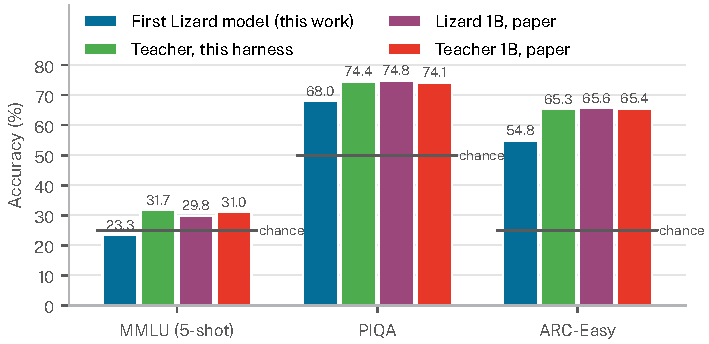
\includegraphics[width=\linewidth]{scores_first_model}
\caption[The first Lizard model against the teacher and the paper]{The first Lizard model against the teacher and the paper. The dark lines show the chance level of each task. Values from \cref{tab:first-scores}.}
\label{fig:first-scores}
\end{figure}

PIQA and ARC-Easy are far above chance (50\% and 25\%). Thus the model still works as a language model. But it is 6.5 points below the teacher on PIQA and 10.5 points on ARC-Easy. The damage is wide. It is not limited to MMLU or to long texts: most PIQA and ARC-Easy prompts are shorter than the 128-token window.

\section{The model selects \enquote{A} on MMLU}
\label{sec:a-collapse}

A score below chance on questions with four options suggests a simple behavior: the model ignores the question and prefers one letter. Then its accuracy in each subject equals the share of that letter among the right answers. \Cref{tab:letters} tests this idea for each letter.

\begin{table}[ht]
\centering
\small
\caption[Accuracy of the first Lizard model against fixed answers]{Accuracy of the first Lizard model against fixed answers on all MMLU questions (\code{letters.py}, project notes, document~7). The real macro mean is 0.233.}
\label{tab:letters}
\begin{tabular}{@{}lrrr@{}}
\toprule
\makecell[l]{If the model\\always gave} & \makecell[r]{Macro\\mean} & \makecell[r]{Mean $|$acc $-$ share$|$\\over subjects} & \makecell[r]{Correlation with\\the accuracy} \\
\midrule
\textbf{\enquote{A}} & \textbf{0.231} & \textbf{0.004} & \textbf{+0.98} \\
\enquote{B} & 0.245 & 0.039 & +0.29 \\
\enquote{C} & 0.254 & 0.051 & $-$0.05 \\
\enquote{D} & 0.270 & 0.087 & $-$0.65 \\
\bottomrule
\end{tabular}
\end{table}

\begin{finding}
On MMLU, the first Lizard model selects \enquote{A} for almost every question. On the MMLU subset, it gives \enquote{A} for 98.6\% of the questions. The accuracy of each subject has a correlation of +0.98 with the share of \enquote{A} as the right answer.
\end{finding}

The question and the four options are usually in the last approximately 100 tokens, inside the window. Thus the collapse is not only a failure of long contexts. The teacher itself is only 6--9 points above chance on MMLU. Thus a model with moderate damage can already fall back to one letter.

\section{The model uses both branches}
\label{sec:ablation}

An earlier idea was that the gated branch did not learn and that the model used only the window. A test removed one branch at inference time and multiplied the other branch by $(1 + \alpha)$. \Cref{tab:ablation} gives the result on PIQA.

\begin{table}[ht]
\centering
\small
\caption[PIQA with one branch removed at inference]{PIQA with one branch removed at inference (\code{ablate.py}, project notes, document~7).}
\label{tab:ablation}
\begin{tabular}{@{}lrr@{}}
\toprule
Model & Accuracy (\%) & Difference \\
\midrule
Full first Lizard model & 67.95 $\pm$ 1.09 & -- \\
Window branch removed: $(1 + \alpha) \cdot$ gated branch & 57.18 $\pm$ 1.15 & $-$10.8 ($z \approx 6.8$) \\
Gated branch removed: $(1 + \alpha) \cdot$ window branch & 52.34 $\pm$ 1.17 & $-$15.6 ($z \approx 9.8$) \\
Chance & 50.0 & \\
\bottomrule
\end{tabular}
\end{table}

Both branches matter. Without the gated branch, the model is almost at chance. This agrees with the design of the paper. Without RoPE, the window cannot find the token order. The gate is the only source of position information. The test measures how much the trained model depends on each branch. It does not show if the architecture needs each branch. The paper tests that question with new training runs (its Table~6).

\section{The gap starts in stage 1}
\label{sec:stage-diff}

The script \code{compare_stages.sh} evaluated the model after stage 1, without LoRA, and after stage 2. \Cref{tab:stage-diff} shows the result. The drop is already present after stage 1. Stage 2 recovers approximately 10 points on PIQA, but MMLU stays near chance. The collapse to \enquote{A} is also present after stage 1. All checkpoints loaded completely: 80 Lizard tensors and 128 LoRA tensors, with 0 missing keys. Thus a loading error does not cause the results.

\begin{table}[ht]
\centering
\small
\caption[The first Lizard model after each stage]{The first Lizard model after each stage (project notes, \enquote{stage difference}).}
\label{tab:stage-diff}
\begin{tabular}{@{}lrrr@{}}
\toprule
Task & After stage 1 & After stage 2 & Teacher \\
\midrule
PIQA & 57.6 $\pm$ 1.2 & 68.0 $\pm$ 1.1 & 74.4 \\
ARC-Easy & 39.0 $\pm$ 1.0 & 54.8 $\pm$ 1.0 & 65.3 \\
MMLU subset & 22.5 (\enquote{A} for 95.4\%) & 24.9 (\enquote{A} for 98.6\%) & 33.7 \\
\bottomrule
\end{tabular}
\end{table}

The gate values give a first explanation. The script measured the gates on one MMLU prompt of 2048 tokens. In layers 1--15, the gate is above 0.999 for all tokens. After 512 tokens, these layers keep at least 95\% of the weight of a token. Thus the gated branch adds up almost all earlier tokens without decay. Only layer 0 has a decay: it keeps 35\% of the weight after 128 tokens. In layer 0, $\alpha$ fell from 1 to 0.042. Thus the window branch of layer 0 has almost no weight. The other layers have $\alpha$ between 0.16 and 0.65. Most sink logits stopped at exact powers of two, such as 0.5, 1.0 and 2.0. This is a sign of bf16 rounding.

\section{The temperature does not change the scores}
\label{sec:temperature}

The harness compares log-likelihoods. A temperature $T$ divides all logits by the same number. This does not change the order of the four letters, so the accuracy must stay the same. \Cref{tab:temperature} confirms this prediction on the stage 1 model.

\begin{table}[ht]
\centering
\small
\caption[The MMLU subset at four temperatures]{The MMLU subset at four temperatures, stage 1 model (project notes, \enquote{temperature}). \enquote{Mass} is the probability of the four letters together. \enquote{Changed} counts the answers that differ from $T = 1$.}
\label{tab:temperature}
\begin{tabular}{@{}rrrrrr@{}}
\toprule
$T$ & Accuracy & \enquote{A} & Changed & Mass & Entropy (bits) \\
\midrule
0.1 & 22.5 & 95.4\% & 0 of 285 & 0.006 & 0.070 \\
0.5 & 22.5 & 95.4\% & 0 of 285 & 0.025 & 0.855 \\
1 & 22.5 & 95.4\% & 0 of 285 & 0.018 & 1.550 \\
2 & 22.5 & 95.4\% & 0 of 285 & 0.002 & 1.879 \\
\bottomrule
\end{tabular}
\end{table}

The test also shows a second problem. The four letters together get only 1.8\% of the probability of the next token at $T = 1$. Thus, for almost all questions, the most probable next token after \enquote{Answer:} is not a letter. The stage 1 model does not follow the answer format of the 5-shot prompt.

\section{Summary of the reproduction}
\label{sec:repro-summary}

\begin{finding}
\textbf{RQ1, first answer.} The first reproduction did not reach the paper. MMLU is 23.3 against 29.8, PIQA 68.0 against 74.8 and ARC-Easy 54.8 against 65.6. The teacher in the same harness gets the expected scores, and the tests of \cref{sec:tests} found no bug. The drop starts in stage 1. On MMLU, the model gives \enquote{A} for almost every question.
\end{finding}

% Chapter 7
\chapter{The Search for the Cause of the Gap}
\label{ch:gap}

This chapter addresses RQ2. It tests the possible causes of the gap one at a time. \Cref{fig:timeline} shows the order of the work.

\begin{figure}[ht]
\centering
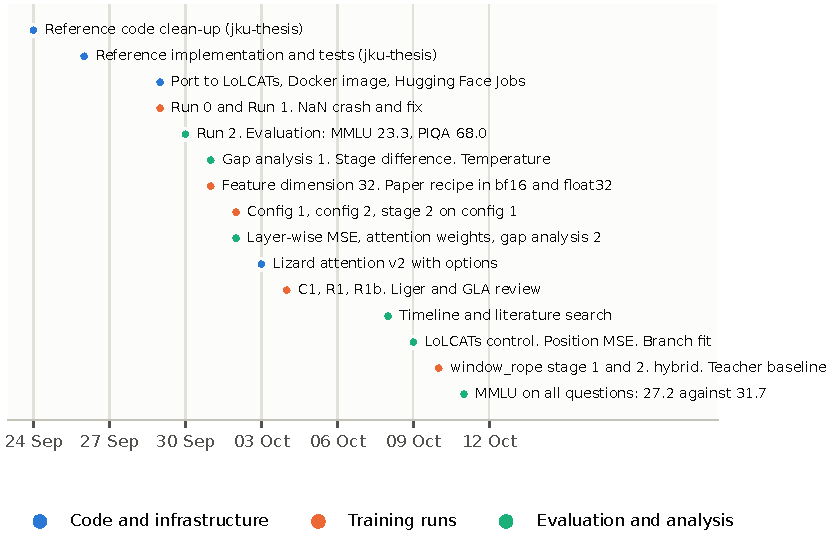
\includegraphics[width=\linewidth]{timeline}
\caption[Timeline of the project]{Timeline of the project, from the pull requests of the two repositories and the project notes (document~18).}
\label{fig:timeline}
\end{figure}

\section{The possible causes}
\label{sec:causes}

The tests of \cref{sec:tests} excluded a bug in the formulas. The first gap analysis ranked the remaining causes (\cref{tab:causes}). The recipe had the largest difference from the paper, so it came first. A missing checkpoint key was cheap to check, so it came next.

\begin{table}[ht]
\centering
\small
\caption[Ranking of the possible causes after the first reproduction]{Ranking of the possible causes after the first reproduction (project notes, document~11), and the later result of each test.}
\label{tab:causes}
\begin{tabularx}{\linewidth}{@{}rLL@{}}
\toprule
\# & Possible cause & Result of the test \\
\midrule
1 & The stage 1 recipe differs from the paper & Not the main cause (\cref{sec:recipe-exp}) \\
2 & The stage 2 recipe and the frozen Lizard parameters & No change in accuracy (\cref{sec:stage2-paper}) \\
3 & Missing keys when the checkpoint loads & Excluded: 0 missing keys in every evaluation \\
4 & The data, the packing or the prompts & Not tested. The data and the packing follow the paper. \\
5 & Numerical effects of bf16 & Real for the recipe of the paper (\cref{sec:precision}) \\
6 & The harness version & Small: the teacher gets the paper values (\cref{tab:teacher}) \\
7 & The tokenization of the MMLU letters & Excluded: each letter is one token \\
8 & The checkpoint selection & Excluded: the best step is the last evaluation in all runs but one \\
9 & The version of the \code{transformers} library & Not tested \\
\bottomrule
\end{tabularx}
\end{table}

\section{Precision: bf16 can discard small updates}
\label{sec:precision}

The first runs store the model and the trainable weights in bf16. This format keeps only approximately 3 significant digits. An AdamW step changes a weight by approximately the learning rate. If the step is smaller than half the distance between two neighboring bf16 numbers, rounding discards it. At the stage 1 learning rate of LoLCATs ($10^{-2}$), rounding discards no updates. At the stage 2 learning rate ($10^{-4}$), it discards 43--65\% of the LoRA updates. At $10^{-3}$, the learning rate of the paper, it discards every update of $\alpha$, because $\alpha$ starts at 1.0.

A stage 1 run with the learning rate and the schedule of the paper showed this effect. In bf16, $\alpha$ stayed at exactly 1.000 in all 16 layers. The validation loss was 8.1641, 2.4 times the loss of the LoLCATs recipe. The same recipe with all weights, the optimizer states and the target in float32 moved $\alpha$ to 0.60--0.79 and lowered the loss to 4.9478. All later runs with the recipe of the paper use float32.

\section{The recipe experiments}
\label{sec:recipe-exp}

Each experiment changed one part of the recipe. These runs use feature dimension 32, the LoLCATs rule for a head dimension of 64. A separate run showed that this value is not a cause. It gave a loss of 3.4219 against 3.2549 for 128, and the gate saturated in the same way. \Cref{tab:recipe-runs} gives the results.

\begin{table}[ht]
\centering
\small
\caption[Stage 1 runs with different recipes]{Stage 1 runs with different recipes (project notes, documents~12 and 14). All runs use the original Lizard attention. Accuracy in \% after stage 1. PIQA has an SE of approximately 1.2 points, and ARC-Easy approximately 1.0 point.}
\label{tab:recipe-runs}
\begin{tabularx}{\linewidth}{@{}Lrrrr@{}}
\toprule
Stage 1 run & Loss & MMLU subset & PIQA & ARC-Easy \\
\midrule
Feature dimension 128, LoLCATs recipe, bf16 (Run 1) & 3.2549 & 22.5 & 57.6 & 39.0 \\
Feature dimension 32, LoLCATs recipe, bf16 & 3.4219 & 23.2 & -- & -- \\
Recipe of the paper, bf16 & 8.1641 & 25.3 & 55.8 & 34.1 \\
Recipe of the paper, float32 & 4.9478 & 24.6 & 57.7 & 35.7 \\
Config 1: also $\beta_2 = 0.99$ and a minimum learning rate & 3.9764 & 26.7 & 57.3 & 36.5 \\
Config 2: config 1 with gradient clipping at 1.0 & 3.5092 & 23.2 & 57.5 & 35.6 \\
\bottomrule
\end{tabularx}
\end{table}

Each step toward the recipe of the paper lowered the loss. With all optimizer settings of Table~13, the recipe of the paper came near the LoLCATs recipe, but it did not pass it. The accuracies stayed in small ranges: 55.8--57.7 on PIQA and 34.1--36.5 on ARC-Easy. With unpaired SEs, none of these differences is clear.

One result was clear. The recipe of the paper stops the saturation of the gate. With the LoLCATs recipe, the gate stays above 0.999 for every token in 14 or 15 of the layers 1--15. With the recipe of the paper, no layer saturates fully. Thus the high learning rate of LoLCATs causes the saturation. But a gate that decays did not give a better model either.

\section{Stage 2 with the recipe of the paper}
\label{sec:stage2-paper}

Stage 2 on config 1 used the stage 2 settings of Table~13 (learning rate $5 \times 10^{-4}$, LoRA on $q$, $k$ and $v$) in float32. Its validation loss was 1.9158, 14.9\% lower than in Run~2 (2.252). But its scores were almost the same: PIQA 67.7 against 67.95, and ARC-Easy 54.9 against 54.8. On the MMLU subset, it gave \enquote{A} for 77.5\% of the questions. \Cref{fig:stage1to2} shows that both stage 2 recipes add approximately 10 points on PIQA and approximately 16--18 points on ARC-Easy. The stage 1 differences did not reach the final model. Stage 2 changed the memory of the gate: in layers 9--15, the weight kept after 512 tokens fell from 0.48--0.94 to below 0.003. The gate parameters stayed frozen. Thus LoRA changed the hidden states that the gate reads.

\begin{figure}[ht]
\centering
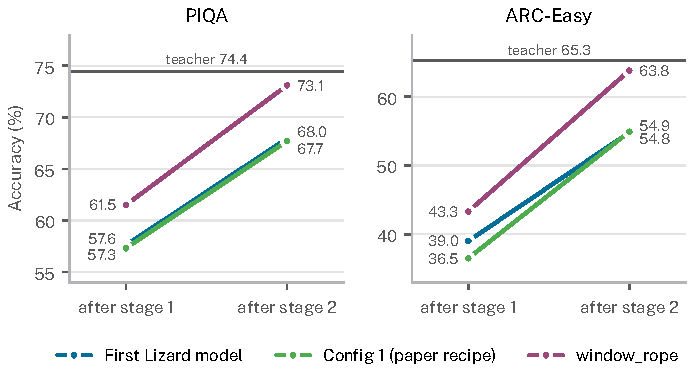
\includegraphics[width=\linewidth]{stage1_to_stage2}
\caption[PIQA and ARC-Easy after stage 1 and after stage 2]{PIQA and ARC-Easy after stage 1 and after stage 2, for three models. The first Lizard model and config 1 end at almost the same values. The \code{window_rope} model of \cref{ch:rope} starts higher and ends higher.}
\label{fig:stage1to2}
\end{figure}

\section{A lower loss does not give a higher accuracy}
\label{sec:loss-vs-acc}

Over the stage 1 runs, the loss fell from 8.16 to 3.05, but PIQA and ARC-Easy did not increase. Over the six runs with ARC-Easy, the rank correlation (Spearman) between the loss and the accuracy is +0.31 for ARC-Easy and $-0.06$ for PIQA. A positive value means that a lower loss comes with a lower accuracy. With six runs, none of these values is clear. \Cref{fig:loss-acc} shows all stage 1 runs of this thesis. Only the runs with RoPE in the window (orange) and the LoLCATs control (green) leave the cluster.

\begin{figure}[ht]
\centering
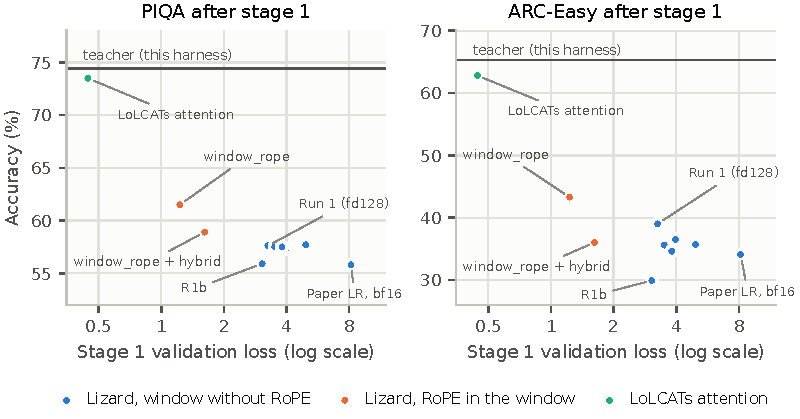
\includegraphics[width=\linewidth]{loss_vs_accuracy}
\caption[Stage 1 loss against the accuracy after stage 1]{Stage 1 loss against the accuracy after stage 1. Each point is one stage 1 run. The unlabeled blue points are the paper recipe in float32, config 1, config 2 and C1. Values in \cref{tab:recipe-runs,tab:v2-runs,tab:control} and Appendix~\ref{app:runs}.}
\label{fig:loss-acc}
\end{figure}

Three properties of the loss can explain this:
\begin{itemize}
\item The loss measures each layer alone, with the input of the teacher. It cannot see an error that grows from layer to layer.
\item All 2048 positions count the same. Positions 0--127 give only 6.25\% of the loss. But almost all PIQA and ARC-Easy prompts are shorter than 128 tokens.
\item Each run has one seed. Thus the noise of the loss and of the scores is not known.
\end{itemize}

\section{A limit for each head}
\label{sec:head-limit}

The second gap analysis looked at the attention weights (\cref{sec:xai-weights}) and found a limit in the architecture. A Lizard row is the gated branch, with weights that sum to 1, plus $\alpha$ times the window branch, with weights that sum to $\rho_i \le 1$. Thus the share of the exact window in a row has an upper limit:
\begin{equation}
\text{window share}_i = \frac{\alpha \rho_i}{1 + \alpha \rho_i} \le \frac{\alpha}{1 + \alpha} .
\label{eq:ceiling}
\end{equation}
All 32 heads of a layer share $\alpha$, the gate, the feature maps and the sink logits. Only $\vq$, $\vk$ and $\vv$ differ between the heads, and stage 1 does not train them. The measurements reach the limit. In layer 15, head 14 of config 1, $\alpha = 0.576$, so the limit is 0.365. The measured window share is 0.365. But the teacher puts 91.3\% of the weight of this head inside the window. In layer 0, the LoLCATs recipe trained $\alpha$ down to 0.063. Then no head of layer 0 can take more than 6\% from the window. But layer 0 has local heads, for example a head that attends to the previous token.

This limit explains several observations. Local teacher heads match worst. All heads of a layer get almost the same long-range share. The training lowers $\alpha$ for the majority of heads, which need far tokens, and the local heads lose. The gated branch cannot become local for one head only, because all heads share one gate. And without RoPE, neither branch knows the relative position of two tokens.

\section{Design options of v2: C1, \code{joint} and \code{hybrid}}
\label{sec:v2-runs}

The options of v2 (\cref{tab:v2-options}) attack the limit. \Cref{tab:v2-runs} gives three runs with the stage 1 recipe of config 1.

\begin{table}[ht]
\centering
\small
\caption[Stage 1 runs with options of Lizard v2]{Stage 1 runs with options of Lizard v2 (project notes, document~13). Accuracy in \% after stage 1.}
\label{tab:v2-runs}
\begin{tabularx}{\linewidth}{@{}Lrrrrr@{}}
\toprule
Run & Loss & PIQA & ARC-Easy & MMLU subset & \enquote{A} \\
\midrule
Config 1 (reference) & 3.9764 & 57.3 & 36.5 & 26.7 & 51.2\% \\
C1: one $\alpha$ for each head & 3.8092 & 57.5 & 34.6 & 23.9 & 64.9\% \\
R1: per-head $\alpha$ and maps, \code{joint} & stopped & -- & -- & -- & -- \\
R1b: per-head $\alpha$ and maps, \code{hybrid}, $\alpha$ start 0.1 & \textbf{3.0542} & 55.9 & \textbf{29.9} & 24.9 & 90.2\% \\
\bottomrule
\end{tabularx}
\end{table}

C1 lowered the loss by 4.2\%, but the accuracy did not change. R1 stopped at 19\% of the first epoch, because \code{joint} gives the gated branch almost no weight at the start values (\cref{tab:proofs}, P6). R1b gave the lowest loss of all Lizard runs at that time, 23.2\% below config 1. But ARC-Easy fell by 6.6 points ($z \approx -4.9$). In layer 15, the shared gate fell to 0.128. Heads 14 and 23 improved by 76--78\%, but 28 of the 32 heads got worse. A short gate gives position information, so it helps local heads. But one gate for all heads takes the long range from the other heads.

\section{The LoLCATs attention as a control}
\label{sec:control}

The control run used the same pipeline, data, recipe and harness, with the original LoLCATs attention in place of Lizard. Thus a clear difference must come from the attention layer. \Cref{tab:control} gives the result.

\begin{table}[ht]
\centering
\small
\caption[The LoLCATs control against Lizard after stage 1]{The LoLCATs control against Lizard after stage 1 (project notes, \enquote{LoLCATs control}). Both runs use the LoLCATs recipe.}
\label{tab:control}
\begin{tabular}{@{}lrrr@{}}
\toprule
Measure & Lizard, Run 1 & LoLCATs control & Difference \\
\midrule
Stage 1 loss & 3.2549 & \textbf{0.4442} & 7.3$\times$ lower \\
PIQA & 57.6 & \textbf{73.5} & +15.9 ($z \approx 10$) \\
ARC-Easy & 39.0 & \textbf{62.8} & +23.8 ($z \approx 17$) \\
MMLU subset & 22.5 & 26.0 & +3.5 ($z \approx 1.0$) \\
\enquote{A} on MMLU & 95.4\% & 19.3\% & -- \\
Probability mass of the four letters & 0.018 & 0.962 & -- \\
\bottomrule
\end{tabular}
\end{table}

After stage 1 alone, the LoLCATs control is above the final first Lizard model on PIQA (+5.5 points) and ARC-Easy (+8.0 points). Thus the pipeline can train a much better model, and the gap comes from the Lizard layer. On short prompts, the control computes almost exactly the teacher attention. Its window has RoPE and covers 128--255 tokens. Its linear part acts only on tokens farther back. Its layer-wise MSE is 3.7 to 36.9 times lower than that of Lizard in every layer. Layer 0 has the largest difference. There, the control gives its window 79\% of the weight on far queries, but Lizard turned its window almost off ($\alpha = 0.042$). MMLU stays near chance for the control too, but the control keeps the answer format: 96.2\% of its probability goes to the four letters.

\section{Summary}
\label{sec:gap-summary}

\begin{finding}
\textbf{RQ2.} The recipe and the precision matter, but they do not explain the gap. bf16 discards small updates and freezes $\alpha$ at the learning rate of the paper. Lower stage 1 losses did not give higher accuracies. The evidence excludes the checkpoint loading, the temperature, the feature dimension and the harness. The LoLCATs control in the same pipeline reaches 98.8\% of the teacher on PIQA after stage 1 alone. Thus the cause is in the Lizard attention. The most probable mechanism is a limit for each head. Its parts are the shared parameters, the gated branch with the weight 1, the ceiling $\alpha/(1+\alpha)$ and the window without RoPE.
\end{finding}

% Chapter 8
\chapter{Analysis with XAI Methods}
\label{ch:xai}

The scores of \cref{ch:repro,ch:gap} show that the model is weak, but not why. This chapter addresses RQ4. It uses four methods that look inside the trained model. All four methods use saved checkpoints, so they need no new training. They ran on the A10 machine.

\section{Layer-wise MSE}
\label{sec:xai-layer}

\textbf{Method.} The script \code{layer_mse.py} runs the stage 1 validation data (16 sequences, 32,768 tokens) through the teacher. Each Lizard layer gets the input of the teacher layer, as in stage 1. The script computes $1000 \times$ MSE for each layer and each head. The sum over the layers gives the stored stage 1 loss again: exactly for the float32 checkpoints, and within 0.1--0.2\% for the bf16 checkpoints. The output of the teacher grows with the depth. Thus the script also gives the \emph{relative} MSE, the MSE divided by the mean square of the teacher output.

\begin{figure}[ht]
\centering
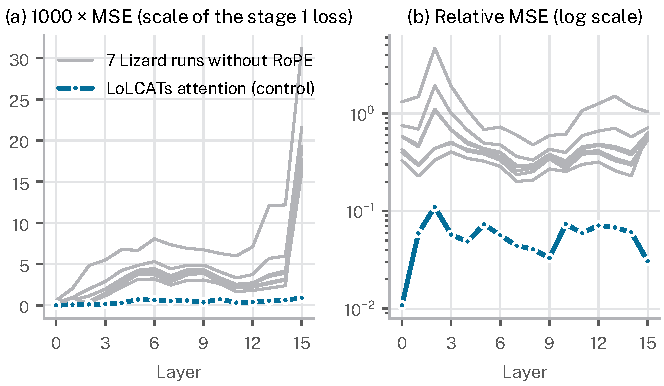
\includegraphics[width=\linewidth]{xai_layer_mse}
\caption[Layer-wise MSE of all Lizard stage 1 runs and the LoLCATs control]{Layer-wise MSE of seven Lizard stage 1 runs (gray) and the LoLCATs control (blue). (a)~$1000 \times$ MSE, the scale of the stage 1 loss. (b)~The MSE divided by the mean square of the teacher output, on a log scale. The control has a lower error in every layer. Data: the JSON files of \enquote{XAI: layer-wise MSE} in the project notes.}
\label{fig:layer-mse}
\end{figure}

\textbf{Findings.} \Cref{fig:layer-mse} shows the result.
\begin{itemize}
\item The MSE is small in the first layers and grows with the depth, as in Figure~14 of the LoLCATs paper. Layer 15 alone gives 24--31\% of the stage 1 loss.
\item Two heads of layer 15, heads 14 and 23, give approximately 20\% of the loss in every Lizard checkpoint.
\item Even with the best recipe, the error has 24--56\% of the power of the teacher output in each layer. With the recipe of the paper in bf16, ten layers have a relative MSE above 1. There, an output of zero would be closer to the teacher.
\item The recipes have the same order in all 16 layers. The difference between them is largest in the first and the last layers.
\item The LoLCATs control has a lower MSE in every layer, against every Lizard checkpoint, by a factor of at least 3.0. Its error has only 1.1--11.0\% of the power of the teacher output.
\item Heads 14 and 23 of layer 15 are not hard for the control. They give 1.9\% of its loss. Thus the teacher heads are not the problem. The Lizard layer is.
\item Layer 0 has the largest ratio between Lizard and the control (30--121 times). This agrees with the control experiment: its window has RoPE and gives the local attention of layer 0.
\end{itemize}

\section{Sample attention weights}
\label{sec:xai-weights}

\textbf{Method.} The script \code{attention_weights.py} computes the full weight matrix of each head for one sample of 1,024 tokens. For Lizard, the matrix is the gated weights plus $\alpha$ times the window weights. A check multiplies the weights with the values and gets the output of the layer again. The script compares each Lizard row with the teacher row. It uses the total variation (TV) distance after it divides the Lizard row by its sum. It also measures the weight outside the window and the weight on the first key. Plots like Figures 18--21 of the LoLCATs paper show the last 32 queries against the first 32 and the last 32 keys.

\begin{figure}[ht]
\centering
\includegraphics[width=0.94\linewidth]{xai-sample-attention-weight/trained_heads0-3_head0}
\caption[Attention weights of head 0 in five layers]{Attention weights of head 0 in five layers. The first row is the teacher. The other rows are three Lizard checkpoints. Each panel shows the last 32 queries against the first 32 keys (left of the dashed line) and the last 32 keys. The teacher has a sharp local pattern in layer 0. All Lizard checkpoints lose it. Source: project notes, \enquote{XAI: sample attention weights}.}
\label{fig:weights}
\end{figure}

\textbf{Findings.}
\begin{itemize}
\item The trained checkpoints reproduce a large part of the teacher weights. Their mean TV distance is 0.31--0.33. The start weights have 0.71.
\item The more local a teacher head is, the worse Lizard matches it. The correlation between the TV distance and the teacher weight outside the window is between $-0.75$ and $-0.78$. Heads with less than 30\% of their weight outside the window have a mean TV distance of 0.56. Heads with more than 70\% have 0.21--0.25.
\item Lizard gives all heads of a layer almost the same long-range share. Inside a layer, the teacher share outside the window has a standard deviation of 0.126 over the heads. For Lizard, it is only 0.034--0.048.
\item Layer 15, head 14 is a local head in the teacher. The teacher puts only 8.7\% of its weight outside the window. Lizard puts 50--53\% there. Its large MSE (\cref{sec:xai-layer}) comes from too much weight far away in Lizard.
\item Layer 0 is the worst layer (TV distance 0.49--0.60). Its head 2 attends to the previous token in the teacher. In all trained checkpoints, this head is almost empty (\cref{fig:weights}). The output of layer 0 is small, so the MSE hardly shows this error.
\end{itemize}

\section{MSE by token position}
\label{sec:xai-position}

\textbf{Method.} The script \code{position_mse.py} splits the query positions into three buckets: 0--127, 128--511 and 512--2047. In the first bucket, all keys are inside the window, as in almost every PIQA and ARC-Easy prompt. The script computes the relative MSE for each layer and bucket. A rank test then compares the error of each bucket with PIQA and ARC-Easy over the checkpoints.

\textbf{Findings.}
\begin{itemize}
\item The LoLCATs control computes the teacher attention at positions 0--127. Its relative MSE there is $8.4 \times 10^{-6}$ to $4.4 \times 10^{-5}$, the size of bf16 rounding.
\item Lizard misses 35--63\% of the teacher output at the same positions (relative MSE 0.351--0.629 over 8 checkpoints). This is more than 20,000 times the value of the control.
\item Layers 2 and 3 have the largest error at short positions. Layer 2 has the largest value in all 8 checkpoints (0.64--1.17).
\item The error at positions 0--127 does not predict PIQA or ARC-Easy over the Lizard checkpoints. The rank correlations are not significant. Thus this error alone cannot rank the stage 1 runs either.
\end{itemize}

The left panel of \cref{fig:position-heatmap} (\cref{ch:rope}) shows this measure for the first Lizard model.

\section{Branch decomposition}
\label{sec:xai-branch}

\textbf{Method.} The script \code{branch_fit.py} asks which branch limits the fit. For each head and each bucket, it fits the teacher output $\vy$ with a weighted sum of candidate outputs by least squares. It reports the remaining error divided by $\|\vy\|^2$. The candidates are:
\begin{itemize}
\item G: the trained gated branch,
\item W: the trained window branch, without RoPE and with the sinks,
\item WR: an oracle window that uses the teacher scores with RoPE over the same 128 keys, without sinks and without trained parameters.
\end{itemize}
The script fits every combination, for example G+W or G+WR. It also reports the error of the trained output. At positions 0--127, WR is the teacher attention, so its error must be only rounding. This is the check of the method: WR gives $1.3 \times 10^{-5}$ in bf16.

\begin{table}[ht]
\centering
\small
\caption[Results of the branch decomposition]{Results of the branch decomposition for the eight Lizard stage 1 checkpoints without RoPE (project notes, \enquote{XAI: branch decomposition}). Values are remaining errors divided by $\|\vy\|^2$.}
\label{tab:branch-fit}
\begin{tabularx}{\linewidth}{@{}LL@{}}
\toprule
Comparison & Result \\
\midrule
W alone, positions 0--127, best weight for each head & 0.394--0.458. The window without RoPE explains only approximately 60\% of the teacher output. \\
G+W against W, positions 0--127 & 0.78--0.81 $\times$. The gated branch helps only a little inside the window. \\
G+WR against WR alone, positions 512--2047 & 0.40--0.58 $\times$. Outside the window, the gated branch gives a large part of the output. \\
G+WR against G+W, all positions & 1.9--2.1 times less error. A window with RoPE would halve the error. \\
Heads 14 and 23 of layer 15, WR alone & 0.017 and 0.134--0.136, against 0.57--0.62 and 0.90--0.94 for the trained output \\
Best weight of G in the G+W fit & Median 0.55--0.81, not 1. The gated branch has too much weight. \\
\bottomrule
\end{tabularx}
\end{table}

\Cref{tab:branch-fit} gives the main results. The two heads with the largest error are window heads. With RoPE in the window, their error would almost disappear. The gated branch is not the main limit: outside the window, it carries the long range. But it has too much weight, because its weights always sum to 1 (\cref{tab:proofs}, P8).

\section{Why short prompts need a good window}
\label{sec:short-prompts}

The write-out files of the harness contain the prompt of each answer option. \Cref{tab:prompt-length} gives the length of the longest option of each question.

\begin{table}[ht]
\centering
\small
\caption[Prompt lengths of PIQA and ARC-Easy]{Prompt lengths of PIQA and ARC-Easy in characters (project notes, document~20). With approximately 4 characters for each token, the 95th percentile is approximately 88 tokens for PIQA and 77 tokens for ARC-Easy.}
\label{tab:prompt-length}
\begin{tabular}{@{}lrrrr@{}}
\toprule
Task & Median & 95th percentile & Maximum & Longer than 512 characters \\
\midrule
PIQA & 132 & 355 & 1,106 & 1.1\% \\
ARC-Easy & 139 & 311 & 802 & 0.3\% \\
\bottomrule
\end{tabular}
\end{table}

Thus for almost every question, all keys are inside the window of 128 tokens. On such a prompt, the teacher computes softmax attention with RoPE over all tokens. The LoLCATs control computes the same, up to rounding. Lizard computes the gated branch over all tokens plus $\alpha$ times the window without RoPE over the same tokens. Thus the window of Lizard must do the work of the teacher, but without RoPE it cannot give the same weights. The gated branch adds weight to tokens that the window already counts.

\section{What the XAI results show together}
\label{sec:xai-summary}

\begin{finding}
\textbf{RQ4, first answer.} The four methods agree. The largest errors are in local heads: head 2 of layer 0 and heads 14 and 23 of layer 15. These heads need exact attention to nearby positions. The window branch without RoPE cannot give it, and the shared gate and $\alpha$ cannot compensate for one head only. The gated branch carries the long range, but it has too much weight at short positions. Ranking for PIQA and ARC-Easy: the window without RoPE is the most probable cause, the gated branch is second, and the Hedgehog maps are third. The direct test is a window with RoPE (\cref{ch:rope}).
\end{finding}

One method did not work as expected: the error at short positions did not predict the accuracy over the Lizard checkpoints (\cref{sec:xai-position}). Thus the XAI methods show the mechanism, but they do not replace the evaluation of each model.

% Chapter 9
\chapter{RoPE in the Window Branch}
\label{ch:rope}

This chapter addresses RQ3. It tests the cause that \cref{ch:xai} found: the window branch without RoPE. The change is one option of v2, \code{window_rope}. All other settings are the settings of Run~1: feature dimension 128, the LoLCATs recipe and bf16. The paper of Lizard writes the window without RoPE. Thus this model is an extension of Lizard, not the reproduction.

\section{Why RoPE in the window, and the predictions}
\label{sec:rope-why}

The branch decomposition gave reference values for Run~1. A conversion of the remaining errors into stage 1 losses gave estimates before the run. The trained output of Run~1 converts to 3.25. The best mix of the two trained branches (G+W) gives 2.96. A window with RoPE alone (WR) gives 2.43. The trained gated branch with a window with RoPE (G+WR) gives 1.20. \Cref{tab:predictions} lists the six predictions and the results.

\begin{table}[ht]
\centering
\small
\caption[Predictions before the \code{window_rope} run and the results]{Predictions before the \code{window_rope} run and the results (project notes, \enquote{RoPE in the window branch}). All six predictions hold.}
\label{tab:predictions}
\begin{tabularx}{\linewidth}{@{}LL@{}}
\toprule
Prediction & Result \\
\midrule
1. The stage 1 loss falls clearly below 3.25, probably below 2.96. & 1.2290. It is also below 2.43, so the trained gated branch adds to the window with RoPE. \\
2. The loss does not reach 1.20, because the gated branch keeps the weight 1. & 1.2290, 2\% above 1.20 \\
3. The relative MSE at positions 0--127 falls clearly from 0.463, but stays above 0. & 0.321 ($-31\%$) \\
4. Layers 0 and 15, and heads 14 and 23 of layer 15, improve most. & Layer 15: 5.3$\times$, layer 0: 3.7$\times$. Heads 14 and 23: 13.7$\times$ and 11.3$\times$. \\
5. $\alpha$ of layer 0 rises above 0.042. & 0.660 \\
6. PIQA and ARC-Easy increase, PIQA by at least 3.2 points. & PIQA +3.9, ARC-Easy +4.3 \\
\bottomrule
\end{tabularx}
\end{table}

\section{What RoPE in the window means for the linearization}
\label{sec:rope-meaning}

RoPE is only in the window branch. The function \code{window_inputs} rotates the queries and keys of the window. The function \code{feature_maps} gets the queries and keys without RoPE. Thus the kernel $\phi(\vq_i)^\top\phi(\vk_t)$ of the gated branch depends only on the content of the tokens.

\textbf{The window branch is not a linear attention.} It is a softmax attention over the last 128 keys and the 4 sinks. Linearization applies only to the gated branch. Thus RoPE in the window does not change the cost or the memory. Each key gets its rotation one time, at its own position, when it goes into the cache. A RoPE score depends only on the distance (\cref{eq:rope}), so the rotated keys in the cache stay valid (\cref{tab:proofs}, P5).

\textbf{Inside the window, the scores are the scores of the teacher.} With RoPE, the window score is $(R_i\vq_i)^\top(R_t\vk_t)/\sqrt{d}$, as in the teacher. Thus for the keys inside the window, the window weights are proportional to the weights of the teacher. Only the denominator differs: it is the sum over the window and the sinks, not over all earlier keys. Without RoPE, the window knows which keys are inside it, but not their order.

\textbf{The two branches get separate tasks.} The window gives the local attention of the teacher. The gated branch must only approximate the part of the teacher output from keys outside the window. Thus the error of the linearization moves to the long range.

\textbf{The gated branch still has no position code.} Its only position information is the decay $\prod \gamma$. In \code{window_rope}, 99.9--100.0\% of the tokens in layers 1--15 have $\gamma > 0.999$. \Cref{fig:gate-decay} shows what this means. If all gates are above 0.999, a token keeps more than $0.999^{128} \approx 0.88$ of its weight after 128 tokens and more than $0.999^{2048} \approx 0.13$ after 2048 tokens. Thus in these layers, the gated branch is almost a mean of the earlier tokens, with weights from the feature similarity. Layer 0 is different: its gate keeps 0.87 of the weight after 128 tokens.

\begin{figure}[ht]
\centering
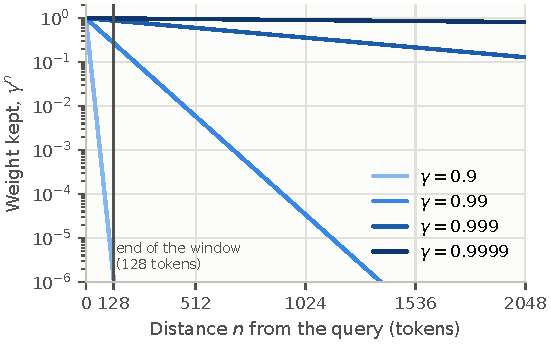
\includegraphics[width=0.66\linewidth]{gate_decay}
\caption[Weight that the gate keeps after $n$ tokens]{Weight $\gamma^n$ that a constant gate keeps after $n$ tokens. In \code{window_rope}, almost all gates of layers 1--15 are above 0.999. Then the gated branch hardly prefers recent tokens.}
\label{fig:gate-decay}
\end{figure}

\Cref{tab:rope-methods} compares the methods. The gated branch could also get RoPE, as in LoLCATs: $\phi(R_i\vq_i)^\top\phi(R_t\vk_t)$. The form stays linear and recurrent. But the Hedgehog map is not linear, so this kernel is not a function of the distance only. The code does not have this option yet.

\begin{table}[ht]
\centering
\small
\caption[Where each method uses RoPE]{Where each method uses RoPE (project notes, document~15 and \enquote{RoPE in the window branch}).}
\label{tab:rope-methods}
\begin{tabularx}{\linewidth}{@{}lLL@{}}
\toprule
Method & Window branch & Linear or gated branch \\
\midrule
LoLCATs & RoPE & RoPE: the feature maps get the queries and keys after RoPE \\
Lizard paper & No RoPE & No RoPE. Position only from the gate. \\
Liger & Paper: no RoPE. Code: RoPE. & No RoPE \\
\code{window_rope} & RoPE & No RoPE. Position only from the gate. \\
\bottomrule
\end{tabularx}
\end{table}

\section{Results after stage 1}
\label{sec:rope-stage1}

\Cref{tab:rope-stage1} gives the scores after stage 1. PIQA and ARC-Easy rise clearly. These are the highest scores of all Lizard stage 1 checkpoints. The loss falls by 62\% and closes 72\% of the gap to the LoLCATs control. But PIQA closes only 25\% of its gap, and ARC-Easy 18\%. The collapse to \enquote{A} on MMLU is mostly gone.

\begin{table}[ht]
\centering
\small
\caption[\code{window_rope} after stage 1]{\code{window_rope} after stage 1 against Run~1 and the LoLCATs control (project notes, \enquote{RoPE in the window branch}). $z$ values with unpaired SEs.}
\label{tab:rope-stage1}
\begin{tabular}{@{}lrrrr@{}}
\toprule
Measure & Run 1 & \code{window_rope} & Difference & LoLCATs control \\
\midrule
Stage 1 loss & 3.2549 & \textbf{1.2290} & $-62\%$ & 0.4442 \\
PIQA & 57.6 $\pm$ 1.2 & \textbf{61.5} $\pm$ 1.1 & +3.9 ($z \approx 2.4$) & 73.5 \\
ARC-Easy & 39.0 $\pm$ 1.0 & \textbf{43.3} $\pm$ 1.0 & +4.3 ($z \approx 3.0$) & 62.8 \\
MMLU subset & 22.5 & 24.6 & +2.1 ($z \approx 0.6$) & 26.0 \\
\enquote{A} on MMLU & 95.4\% & 40.0\% & -- & 19.3\% \\
$\alpha$ of layer 0 & 0.042 & 0.660 & -- & -- \\
\bottomrule
\end{tabular}
\end{table}

\Cref{fig:rope-layer} shows that the MSE falls in every layer, most of all in layers 15 and 0. Heads 14 and 23 of layer 15 now give 4.4\% of the loss, against 21\% in Run~1. For the first time, a Lizard checkpoint has less than 3.0 times the MSE of the control in some layers (10 of 16).

\begin{figure}[ht]
\centering
\includegraphics[width=\linewidth]{window-rope/layer_mse_vs_run1}
\caption[Layer-wise MSE of \code{window_rope} against Run~1]{Layer-wise MSE of \code{window_rope} (orange) against Run~1 (blue). Panel (b) shows the difference. Source: project notes, \enquote{RoPE in the window branch}.}
\label{fig:rope-layer}
\end{figure}

The branch decomposition explains why the accuracy rose less than the loss (\cref{fig:rope-branch}). At positions 0--127, the window with RoPE alone now keeps an error of only 0.048 (Run~1: 0.403). The rest comes from the sinks. But the trained output has an error of 0.321 there, while the best mix of the same two branches has 0.025. Thus at short positions, the \emph{mix} of the branches gives most of the error. The best weight of the gated branch is 0.08 at positions 0--127, 0.65 at positions 128--511 and 0.79 at positions 512--2047. With \code{gla_norm: row}, the gated branch keeps the weight 1 at every position. In the stage 1 loss, 94\% of the positions are above 127. Thus the training sets the mix for long contexts, and the short prompts of PIQA and ARC-Easy get a mix that does not fit them.

\begin{figure}[ht]
\centering
\includegraphics[width=\linewidth]{window-rope/branch_fit_0-127}
\caption[Branch decomposition at positions 0--127]{Branch decomposition at positions 0--127 for Run~1 (left) and \code{window_rope} (right). Each cell is the remaining error after the best fit of a set of branches. In \code{window_rope}, the window W alone is almost exact (light cells), but the trained output (last column) is not. Source: project notes, \enquote{RoPE in the window branch}.}
\label{fig:rope-branch}
\end{figure}

\begin{figure}[ht]
\centering
\includegraphics[width=0.72\linewidth]{window-rope/position_heatmap}
\caption[Relative MSE by layer and position bucket]{Relative MSE by layer and position bucket for Run~1 (left) and \code{window_rope} (right). Short positions now have the largest error, most of all in layers 2 and 3. Source: project notes, \enquote{RoPE in the window branch}.}
\label{fig:position-heatmap}
\end{figure}

\section{Results after stage 2}
\label{sec:rope-stage2}

Stage 2 trained only the LoRA weights, as in Run~2. Its validation loss fell from 1.3432 to 1.2352, against 2.252 for Run~2. \Cref{tab:rope-stage2} gives the scores.

\begin{table}[ht]
\centering
\small
\caption[\code{window_rope} after stage 2]{\code{window_rope} after stage 2 (project notes, \enquote{RoPE in the window branch}, Run~2, and document~7, section~6). Accuracy in \%.}
\label{tab:rope-stage2}
\begin{tabular}{@{}lrrrr@{}}
\toprule
Task & \makecell[r]{First Lizard\\model} & \code{window_rope} & Difference & \makecell[r]{Teacher,\\this harness} \\
\midrule
PIQA & 67.95 $\pm$ 1.09 & \textbf{73.1} $\pm$ 1.0 & +5.1 ($z \approx 3.4$) & 74.4 $\pm$ 1.0 \\
ARC-Easy & 54.8 $\pm$ 1.0 & \textbf{63.8} $\pm$ 1.0 & +9.0 ($z \approx 6.3$) & 65.3 $\pm$ 1.0 \\
MMLU subset & 24.9 & 25.6 & +0.7 & 33.7 \\
MMLU, all questions & 23.3 & \textbf{27.2} $\pm$ 0.4 & +3.9 & 31.7 $\pm$ 0.4 \\
Stage 2 validation loss & 2.252 & 1.235 & -- & -- \\
\bottomrule
\end{tabular}
\end{table}

\begin{figure}[ht]
\centering
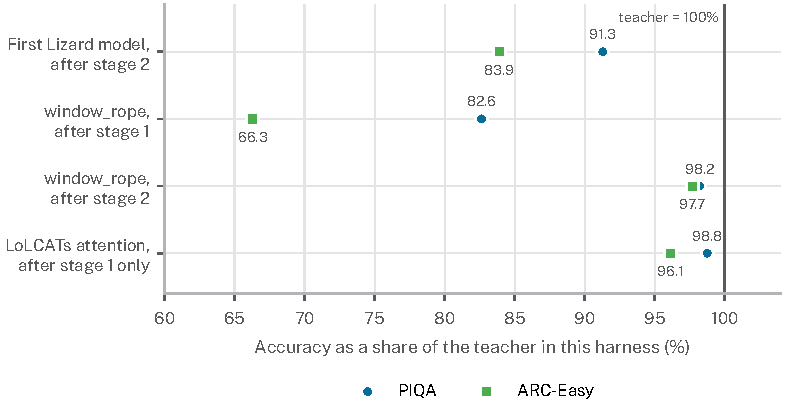
\includegraphics[width=\linewidth]{percent_of_teacher}
\caption[PIQA and ARC-Easy as a share of the teacher]{PIQA and ARC-Easy as a share of the teacher in this harness (74.43 and 65.32). After stage 2, \code{window_rope} reaches 98.2\% and 97.7\%. The LoLCATs control reaches a similar level after stage 1 alone.}
\label{fig:percent}
\end{figure}

\begin{finding}
After stage 2, \code{window_rope} is the best Lizard model of this work. It gets 98.2\% of the teacher on PIQA and 97.7\% on ARC-Easy (\cref{fig:percent}). The differences to the teacher are $-1.4$ points ($z \approx -0.9$) and $-1.5$ points ($z \approx -1.1$), so they are not clear. The gain of stage 1 grows in stage 2: from +3.9 to +5.1 points on PIQA, and from +4.3 to +9.0 points on ARC-Easy.
\end{finding}

\section{The shared denominator does not help}
\label{sec:hybrid}

The mix problem of \cref{sec:rope-stage1} suggested the next step: the shared denominator of LoLCATs (\code{gla_norm: hybrid}). With this option, the share of the gated branch can grow with the position. The run started $\alpha$ at 0.1, as LoLCATs does. \Cref{tab:hybrid} gives the result.

\begin{table}[ht]
\centering
\small
\caption[\code{window_rope} with and without \code{hybrid}]{\code{window_rope} with and without \code{hybrid}, after stage 1 (project notes, \enquote{\code{window_rope} with the shared denominator}).}
\label{tab:hybrid}
\begin{tabular}{@{}lrrr@{}}
\toprule
Measure & \code{window_rope} & with \code{hybrid} & Difference \\
\midrule
Stage 1 loss & \textbf{1.2290} & 1.6172 & +32\% \\
PIQA & \textbf{61.5} & 58.9 & $-2.6$ ($z \approx -1.6$) \\
ARC-Easy & \textbf{43.3} & 36.0 & $-7.3$ ($z \approx -5.1$) \\
MMLU subset & 24.6 & 25.3 & +0.7 \\
Relative MSE, positions 0--127 & 0.321 & \textbf{0.222} & $-31\%$ \\
\bottomrule
\end{tabular}
\end{table}

The gate split the layers into two groups. In 7 layers, the gate stayed open, and the MSE fell at all positions. In layer 0, the MSE fell 5.8 times. In the other 9 layers, the gate closed: $\gamma$ fell below 0.001 for almost all tokens, so the gated branch kept only the current token. These 9 layers lost the long range. Their MSE was 1.8--2.7 times that of \code{window_rope}, and they gave 78\% of the loss. The error at short positions fell, but PIQA and ARC-Easy fell too. Thus \code{window_rope} with \code{row} stayed the best setting.

\section{Table 9 of the paper}
\label{sec:table9}

\Cref{tab:table9} compares \code{window_rope} with Table~9 of the paper. The paper used a newer harness, so only the teacher rows of the same harness give the real gap. ARC-Challenge and HellaSwag ran on 2026-10-11. WinoGrande has no result yet.

\begin{table}[ht]
\centering
\small
\caption[\code{window_rope} against Table 9 of the paper]{\code{window_rope} after stage 2 against Table~9 of the paper. Accuracy in \%. ARC-Challenge, HellaSwag and WinoGrande use \code{acc_norm}, \code{acc_norm} and \code{acc}, as in the paper.}
\label{tab:table9}
\setlength{\tabcolsep}{4pt}
\begin{tabular}{@{}lrrrrrr@{}}
\toprule
Model & PIQA & ARC-e & ARC-c & \makecell[r]{Hella-\\Swag} & \makecell[r]{Wino-\\Grande} & MMLU \\
\midrule
Teacher, this harness & 74.4 & 65.3 & -- & -- & -- & 31.7 \\
\code{window_rope}, this harness & 73.1 & 63.8 & 36.1 & 60.7 & pending & 27.2 \\
\midrule
Teacher, paper & 74.1 & 65.4 & 36.4 & 63.8 & 60.0 & 31.0 \\
LoLCATs, paper & 74.6 & 63.0 & 35.1 & 63.7 & 61.5 & 27.3 \\
Lizard, paper & 74.8 & 65.6 & 36.5 & 64.1 & 59.7 & 29.8 \\
\bottomrule
\end{tabular}
\end{table}

On ARC-Challenge, \code{window_rope} gets 36.1 with \code{acc_norm} (33.2 with \code{acc}). This is within 0.4 points of the paper values for the teacher and for Lizard. On HellaSwag, it gets 60.7 $\pm$ 0.5 with \code{acc_norm} (47.1 with \code{acc}). This is 3.1 points below the teacher of the paper (63.8), a larger gap than on the other short tasks. The teacher of this harness has no value on these tasks yet. If the two harness versions agree here as on PIQA and ARC-Easy, \code{window_rope} keeps approximately 95\% of the teacher on HellaSwag.

\section{MMLU on all questions}
\label{sec:mmlu-full}

The MMLU subset has an SE of 2.6 points. Thus both models also ran on all 14,042 questions (\cref{tab:mmlu-full}).

\begin{table}[ht]
\centering
\small
\caption[MMLU on all questions]{MMLU on all questions, 5-shot (project notes, \enquote{RoPE in the window branch}, findings 15--21).}
\label{tab:mmlu-full}
\begin{tabular}{@{}lrr@{}}
\toprule
Measure & Teacher & \code{window_rope} \\
\midrule
Mean over the subjects & \textbf{31.7} $\pm$ 0.4 & \textbf{27.2} $\pm$ 0.4 \\
Mean over the questions & 31.0 & 26.9 \\
Probability mass of the four letters & 0.999 & 0.975 \\
Confidence (largest letter probability) & 0.342 & 0.354 \\
Entropy over the four letters & 1.904 bits & 1.900 bits \\
\bottomrule
\end{tabular}
\end{table}

\textbf{The model is above chance, but it keeps only one third of the knowledge.} 27.2 is approximately 5.9 SE above 25\%. The first Lizard model was 4.8 SE below. On the same questions, the teacher has 4.2 more points (paired SE 0.44, $z \approx 9.5$). The teacher alone is right on 2,210 questions, and the student alone on 1,625 (McNemar $z \approx 9.5$). The student gets 86\% of the teacher score, but only 33\% of the part of the teacher score above chance: $(27.2 - 25)/(31.7 - 25)$.

\textbf{The student follows the teacher.} When the teacher is right, the student is right on 49.3\% of the questions. When the teacher is wrong, the student is right on only 16.8\%. Without a link between the models, both values would be 26.9\%.

\textbf{The student loses most where the teacher knows most.} \Cref{fig:mmlu-groups} shows the four subject groups. The gap is 2.8 and 2.7 points in STEM and the humanities, where the teacher is near chance. It is 4.7 and 7.2 points in the social sciences and the group \enquote{other}, where the teacher knows more. \Cref{fig:mmlu-subjects} shows the same pattern for the single subjects.

\begin{figure}[ht]
\centering
\begin{minipage}[t]{0.6\linewidth}
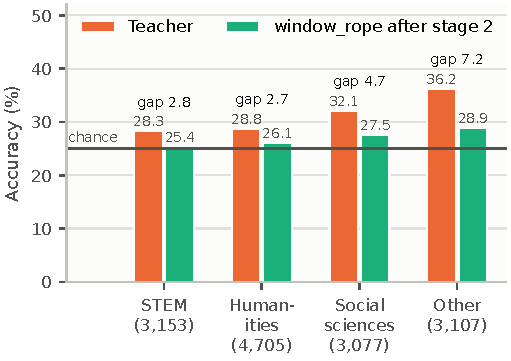
\includegraphics[width=\linewidth]{mmlu_groups}
\caption[MMLU by subject group]{MMLU by subject group, with the number of questions. The values are means over the questions of each group.}
\label{fig:mmlu-groups}
\end{minipage}\hfill
\begin{minipage}[t]{0.37\linewidth}
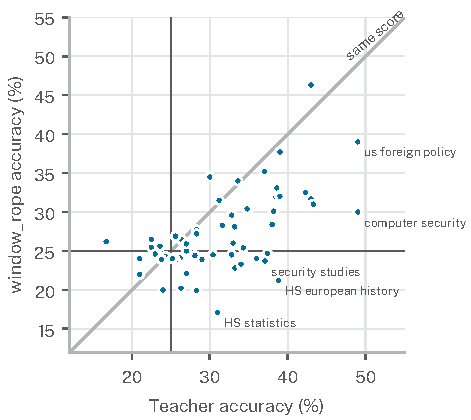
\includegraphics[width=\linewidth]{mmlu_subjects}
\caption[MMLU for each subject]{MMLU for each of the 57 subjects. Points below the diagonal are subjects where the student loses. Data in Appendix~\ref{app:mmlu}.}
\label{fig:mmlu-subjects}
\end{minipage}
\end{figure}

\textbf{The gap does not grow with the prompt length.} In the four quarters of the prompt length, the gap is 5.9, 3.8, 2.4 and 4.5 points. The shortest prompts have the largest gap. The length and the subject are not independent, but this result does not support the idea that the long 5-shot context causes the gap.

\section{Letters and ties on MMLU}
\label{sec:ties}

\Cref{fig:mmlu-letters} shows the letters that the two models select. Both models prefer \enquote{A} and almost never give \enquote{D}. Thus the even spread over the letters is a property of the 1B teacher in this format, not a sign of damage in the student. The gap is in the choice of the right letter.

\begin{figure}[ht]
\centering
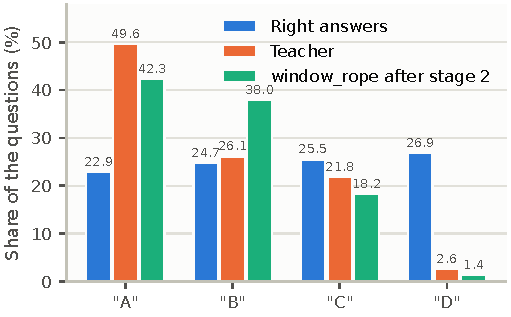
\includegraphics[width=0.66\linewidth]{mmlu_letters}
\caption[Selected letters on all MMLU questions]{Selected letters on all MMLU questions, and the share of each letter among the right answers.}
\label{fig:mmlu-letters}
\end{figure}

The letter log-likelihoods of both models are multiples of 0.125 or 0.25, because the logits are in bf16. Thus ties at the maximum are common: 24.2\% of the teacher answers and 20.5\% of the student answers. In a tie, the harness selects the first letter. Suppose that a random choice breaks each tie. Then the mean over the questions is 31.7 for the teacher (stored 31.0) and 27.0 for the student (stored 26.9). The ties add to the preference for \enquote{A}, but the rare \enquote{D} does not come from the ties.

\begin{finding}
\textbf{RQ3.} RoPE in the window branch closes almost all of the gap on PIQA and ARC-Easy. It does not close the gap on MMLU: 27.2 against 31.7 for the teacher. The shared denominator does not help, because the gate closes in 9 of 16 layers.
\end{finding}

% Chapter 10
\chapter{Discussion}
\label{ch:discussion}

\section{Answers to the research questions}
\label{sec:answers}

\begin{description}[leftmargin=1.2cm,style=nextline]
\item[RQ1] \textbf{Can the Lizard results for Llama-3.2-1B be reproduced?} Not with the method as written. The first Lizard model got 23.3 on MMLU, 68.0 on PIQA and 54.8 on ARC-Easy, against 29.8, 74.8 and 65.6 in the paper (\cref{ch:repro}). The extension \code{window_rope} comes close on PIQA and ARC-Easy, but it is not the method of the paper.
\item[RQ2] \textbf{Which differences explain the gap?} Not the recipe alone and not the code. The tests found no bug. The recipe of the paper in float32 did not give a better model than the LoLCATs recipe. The LoLCATs control in the same pipeline reached the teacher on short tasks after stage 1. Thus the attention layer causes most of the gap (\cref{ch:gap}).
\item[RQ3] \textbf{Which changes close the gap?} RoPE in the window branch closes most of the gap on PIQA and ARC-Easy: 98.2\% and 97.7\% of the teacher. ARC-Challenge reaches the paper values. HellaSwag stays 3.1 points below the teacher of the paper. One $\alpha$ for each head, feature maps for each head and the shared denominator did not help (\cref{ch:gap,ch:rope}).
\item[RQ4] \textbf{Do the measurements inside the model explain the scores?} Partly. They found the mechanism: local heads, a window without RoPE and a gated branch with too much weight at short positions. They predicted the effect of RoPE in the window correctly. But the error at short positions did not rank the checkpoints by accuracy (\cref{ch:xai}).
\end{description}

\section{Why PIQA and ARC-Easy recover, and MMLU does not}
\label{sec:why-mmlu}

PIQA and ARC-Easy prompts are short, so the window does almost all the work. A window with RoPE computes the teacher scores inside the window. Thus these two tasks mostly test the window, and \code{window_rope} reaches the teacher. MMLU is different in three ways. The 5-shot prompts have up to 2048 tokens, so the gated branch acts on most of the context. The task tests knowledge, and the teacher itself is only 6.7 points above chance. And the answer is one letter, so the model must connect the right option with its letter. Bick et al.~\cite{bick2025} explain that a few sharp retrieval heads do this step, and that recurrent models give smoother attention. This agrees with the results, but the project did not test it directly.

The full MMLU results add two facts. First, the student follows the teacher: it is right much more often when the teacher is right. Thus the student keeps part of the knowledge. Second, the gap does not grow with the prompt length. Thus the long context alone does not explain the gap. The stage 2 data may also matter: stage 2 uses the next-token loss on Alpaca, not the logits of the teacher.

\section{Differences from the paper that stay}
\label{sec:differences}

Some differences from the paper remain. The paper has no public code. The open points D1, D2, D3 and D5 (\cref{tab:open-points}) allow other readings. The evaluation harness is older than the harness of the paper, although the teacher scores agree within 0.7 points. A web search found an ACL 2026 version of the paper. Its abstract reports MMLU gains of 9.4--24.5 points, but this work did not read its tables. The Liger code applies RoPE in the window although the Liger paper does not write it. Thus the code of the Lizard authors may also differ from their paper. This is a possibility, not a fact. A message to the authors is the direct way to find out.

\section{Limits of this study}
\label{sec:limits}

\begin{itemize}
\item \textbf{One seed.} Each run has one random seed. Thus the variance from run to run is not known, and small differences between runs can be noise.
\item \textbf{Small question sets.} Many early decisions used the MMLU subset, with an SE of 2.6 points. Only the final models ran on all questions.
\item \textbf{bf16 ties.} The bf16 logits give ties in 20--24\% of the MMLU answers, and the harness then selects the first letter. This changes the accuracy by up to 0.7 points.
\item \textbf{Unpaired statistics.} Most comparisons use unpaired SEs. Paired tests would be more sensitive.
\item \textbf{No efficiency measurement.} The code is a dense reference that materializes $L \times L$ matrices. This thesis does not measure the speed or the memory of the trained model on long inputs.
\item \textbf{Unchecked sources.} Some related work comes from web searches and from ChatGPT answers. The full texts of these sources were not read.
\end{itemize}

\section{Lessons for reproduction work}
\label{sec:lessons}

\begin{enumerate}
\item \textbf{Test the code first.} The tests against a slow reference excluded a whole class of causes in a short time.
\item \textbf{Change one thing at a time.} Each experiment changed one setting. Thus each result has a clear cause.
\item \textbf{Measure the accuracy, not only the loss.} The stage 1 loss fell from 8.16 to 3.05 over the runs, but the accuracy did not rise.
\item \textbf{Use a control.} The LoLCATs control showed in one run that the pipeline works and that the attention layer is the cause.
\item \textbf{Read the code of related methods, not only their papers.} The RoPE in the window of the Liger code was an important hint.
\end{enumerate}

% Chapter 11
\chapter{Conclusion and Future Work}
\label{ch:conclusion}

\section{Summary}
\label{sec:summary}

This thesis reproduced the Lizard linearization on Llama-3.2-1B in the open LoLCATs code base. The first model stayed far below the paper, and on MMLU it gave \enquote{A} for almost every question. Tests excluded a bug in the formulas. Experiments with the recipe, the precision and the readings of the paper lowered the stage 1 loss, but they did not raise the accuracy. A control with the LoLCATs attention showed that the cause is in the Lizard layer. Four interpretability methods found the most probable mechanism: the window branch without RoPE cannot reproduce the local heads of the teacher. With RoPE in the window, the model reaches 98.2\% of the teacher on PIQA and 97.7\% on ARC-Easy. On MMLU, it gets 27.2 against 31.7 for the teacher.

\section{Future work}
\label{sec:future}

\begin{enumerate}
\item \textbf{Complete Table 9.} Evaluate ARC-Challenge, HellaSwag and WinoGrande for the teacher in the same harness, and WinoGrande for \code{window_rope}.
\item \textbf{Checks on MMLU without training.} Evaluate MMLU 0-shot, with a beginning-of-text token, with rotated options and without the gated branch. These checks separate a loss of knowledge from a failure of the letter step.
\item \textbf{Softmax layers or heads.} Keep one or two layers as softmax, selected by the KL divergence or by a search for G\&A heads~\cite{bick2025,klselect}. LoLCATs and Lizard report large MMLU gains with such hybrids at 8B.
\item \textbf{A KL loss in stage 2.} Train stage 2 on the logits of the teacher, as RADLADS~\cite{radlads} does.
\item \textbf{Less gated weight at short positions.} Give the gated branch only the keys outside the window. Another way is to start the gate near 0.95 with the shared denominator, so that the gates do not close.
\item \textbf{RoPE in the gated branch.} Test $\phi(R_i\vq_i)^\top\phi(R_t\vk_t)$ as a new option.
\item \textbf{More seeds and an efficiency benchmark.} Repeat the best run with other seeds. Measure the speed and the memory for long inputs with a chunked kernel.
\item \textbf{A hyperparameter search.} The project notes plan an Optuna study with the mean of PIQA and ARC-Easy as its score.
\end{enumerate}


\cleardoubleoddpage
\printbibliography

\appendix
% Appendix A
\chapter{Definitions}
\label{app:definitions}

This appendix gives short definitions of terms that the thesis uses.

\begin{description}[leftmargin=0.6cm,style=nextline]
\item[Causal language modeling] Training a model to predict the next token from the earlier tokens. The loss is the cross-entropy of the right next token. Stage 2 uses this loss.
\item[Fine-tuning] More training of a trained model on new data, often with a small learning rate or with few trainable parameters.
\item[Token] A piece of text, for example a word or a part of a word. The model reads and writes tokens.
\item[Context size] The number of tokens that the model reads at one time. The training of this thesis uses 2048 tokens.
\item[Packing] Joining many short examples into one long sequence, so that no space is lost. Each training sequence of this thesis has exactly 2048 tokens from several Alpaca examples.
\item[EOS token] A special token that marks the end of a text. With packing, it separates the examples in a sequence.
\item[BOS token] A special token at the beginning of a text. The harness of this thesis does not add it for Llama.
\item[Padding] Extra tokens that make short sequences as long as the longest sequence of a batch. The model must ignore them.
\item[Batch and gradient accumulation] A batch is the set of sequences for one gradient step. With gradient accumulation, the trainer adds the gradients of several small batches before it makes one step. This thesis uses 1 sequence and 8 accumulation steps.
\item[Epoch] One pass over all training data.
\item[Learning rate schedule] The rule that changes the learning rate during training. \emph{Warmup} increases it from a small value at the start. A \emph{cosine} schedule then decreases it along a cosine curve. \emph{Reduce on plateau} decreases it only when the validation loss stops improving.
\item[Gradient clipping] A limit on the norm of the gradient. A larger gradient gets a smaller scale before the step.
\item[bf16 and float32] Two number formats. float32 has 24 bits of precision. bf16 has 8 bits of precision, but the same range as float32. bf16 needs half the memory. But it cannot store small changes to a weight.
\item[Log-likelihood] The logarithm of the probability that the model gives to a text. The harness uses it to compare answer options.
\item[Few-shot] A prompt with some solved examples before the question. MMLU in this thesis uses 5 examples (5-shot).
\item[Standard error] The expected spread of a measured value around its true value. For an accuracy $p$ on $n$ questions, it is $\sqrt{p(1-p)/n}$.
\end{description}

% Appendix B
\chapter{Formulas and Proof Sketches}
\label{app:formulas}

This appendix gives short derivations for the main claims of \cref{tab:proofs}. The project notes (documents~13, 14 and 15) give the full audits and the float64 checks.

\section{The parallel form equals the recurrent form (P1)}

Let $\vS_0 = 0$ and $\vS_i = \gamma_i \vS_{i-1} + \phi_k(\vk_i)\vv_i^\top$. By induction over $i$,
\begin{equation}
\vS_i = \sum_{t=1}^{i} \left( \prod_{l=t+1}^{i} \gamma_l \right) \phi_k(\vk_t)\, \vv_t^\top .
\end{equation}
The step from $i-1$ to $i$ multiplies every term by $\gamma_i$ and adds the term $t = i$, with an empty product equal to 1. Thus $\phi_q(\vq_i)^\top \vS_i$ is the numerator of \cref{eq:gla}. A second state $\vz_i = \gamma_i \vz_{i-1} + \phi_k(\vk_i)$ gives the denominator in the same way. The denominator is at least $\phi_q(\vq_i)^\top\phi_k(\vk_i) > 0$, because all features are positive. The float64 check gave a difference of $2.2 \times 10^{-16}$.

\section{The total weight of a row and the window share (P2, P8)}

The gated weights of row $i$ sum to 1, because the branch divides by its own row sum. The window weights sum to
\begin{equation}
\rho_i = \frac{\sum_{t \in W_i} e^{s_{it}}}{\sum_{j} e^{t_j} + \sum_{t \in W_i} e^{s_{it}}} \le 1 .
\end{equation}
Thus the total weight of the row is $1 + \alpha\rho_i$. For $\alpha \ge 0$, the share of the window is $\alpha\rho_i / (1 + \alpha\rho_i)$. This value grows with $\alpha\rho_i$, so it is at most $\alpha/(1 + \alpha)$. With one $\alpha$ for each head (C1), the limit becomes $\alpha_h/(1+\alpha_h)$ for each head. Without the denominator in the gated branch, the limit disappears.

\section{Four equal sinks act as one sink (P7)}

The sinks enter the loss only through $\sum_j \exp(t_j)$. Thus equal logits get equal gradients. Adam updates each element from its own history of gradients. Equal histories give equal updates, so by induction the logits stay equal. Then $\sum_{j=1}^{4} e^{t} = e^{t + \ln 4}$, which is one sink with the logit $t + \ln 4$. All runs of this thesis show four equal sink logits in each layer.

\section{The written sink term can break the denominator (P4)}

The paper writes $\sum_j t_j$ in the denominator. With $m = 4$ sinks, one key with the score 0 and $t_j = -0.25$ for all $j$, the denominator is $4 \cdot (-0.25) + e^0 = 0$. With $t_j = -1$, it is $-3$. With $\sum_j \exp(t_j)$, the denominator is always positive.

\section{The log-space form and the softmax map (P3)}

The log-space form adds $\log c_t$ to the argument of the feature map. For the $\exp$ map, $\exp(\vx W + \log c_t) = c_t \exp(\vx W)$, which gives the gate product. For the softmax map, the same constant appears in every element of the softmax and cancels: $\mathrm{softmax}(\vx W + \log c_t) = \mathrm{softmax}(\vx W)$. Thus with the softmax map of Table~13, the gate disappears from this form.

\section{The shared denominator (\code{hybrid})}

Let $w_{it} = c_{it}\,\phi_q(\vq_i)^\top\phi_k(\vk_t)$ be the gated weights and $m_i$ the larger of the largest window score and the largest sink logit. The option \code{hybrid} computes
\begin{equation}
\vy_i = \frac{\sum_{t \le i} w_{it}\, \vv_t + |\alpha| \sum_{t \in W_i} e^{s_{it} - m_i}\, \vv_t}{\sum_{t \le i} w_{it} + |\alpha| \left( \sum_{t \in W_i} e^{s_{it} - m_i} + \sum_j e^{t_j - m_i} \right)} .
\end{equation}
The row is a weighted mean of the values with a total weight below 1. The share of the gated branch is its part of the denominator. If the gates are 1, the gated sum grows with the position $i$, but the window sum has at most 128 terms. Thus the window share falls approximately as $1/i$ (P9).

% Appendix C
\chapter{Configurations of the Runs}
\label{app:configs}

Each run uses three config files of the LoLCATs code base. The model config is in \code{configs/model}. The distill config for stage 1 and the finetune config for stage 2 are in \code{configs/experiment}. \Cref{tab:configs} lists them.

{\small
\begin{longtable}{@{}>{\raggedright\arraybackslash}p{2.9cm}>{\raggedright\arraybackslash}p{5.6cm}>{\raggedright\arraybackslash}p{6.0cm}@{}}
\caption[Config files of the runs]{Config files of the runs. All model configs start with \code{distill_llama3_2_1b_lizard}, which the table writes as \code{...}.}\label{tab:configs}\\
\toprule
Run & Model config & Stage 1 / stage 2 config \\
\midrule
\endfirsthead
\toprule
Run & Model config & Stage 1 / stage 2 config \\
\midrule
\endhead
\bottomrule
\endfoot
Run 1 and Run 2 & \nolinkurl{..._w128_fd128_m4} & \nolinkurl{..._lr1e-2_1b} / \nolinkurl{finetune_lora_qkvo_alpaca_clean_1b} \\
Feature dimension 32 & \nolinkurl{..._w128_fd32_m4} & \nolinkurl{..._lr1e-2_1b} \\
Paper LR, bf16 & \nolinkurl{..._w128_fd32_m4} & \nolinkurl{..._lr1e-3_cosine_1b} \\
Paper LR, float32 & \nolinkurl{..._w128_fd32_m4_fp32} & \nolinkurl{..._lr1e-3_cosine_1b} \\
Config 1 & \nolinkurl{..._w128_fd32_m4_fp32} & \nolinkurl{..._lr1e-3_paper_noclip_1b} / \nolinkurl{finetune_lora_qkv_alpaca_clean_paper_noclip_1b} \\
Config 2 & \nolinkurl{..._w128_fd32_m4_fp32} & \nolinkurl{..._lr1e-3_paper_1b} \\
C1 & \nolinkurl{..._v2_w128_fd32_m4_fp32_alphahead} & \nolinkurl{..._lr1e-3_paper_noclip_1b} \\
R1 & \nolinkurl{..._v2_w128_fd32_m4_fp32_perhead_joint} & \nolinkurl{..._lr1e-3_paper_noclip_1b} \\
R1b & \nolinkurl{..._v2_w128_fd32_m4_fp32_perhead_hybrid} & \nolinkurl{..._lr1e-3_paper_noclip_1b} \\
\code{window_rope} & \nolinkurl{..._v2_w128_fd128_m4_windowrope} & \nolinkurl{..._lr1e-2_1b} / \nolinkurl{finetune_lora_qkvo_alpaca_clean_1b} \\
\code{window_rope} + \code{hybrid} & \nolinkurl{..._v2_w128_fd128_m4_windowrope_hybrid} & \nolinkurl{..._lr1e-2_1b} \\
LoLCATs control & \nolinkurl{distill_llama3_1_1b_lk_smd_wtk64_fd64_w01} & \nolinkurl{..._lr1e-2_1b} \\
\end{longtable}
}

The distill configs start with \code{distill_alpaca_clean_xent0_mse1000}. The table writes this part as \code{...} too. The model config of the LoLCATs control sets the window to 128 and the feature dimension to 128, although its name says 64.

The main settings of the model config of \code{window_rope}:
\begin{verbatim}
attention:
  attention_type: lolcats_llama_lizard_v2
  feature_dim: 128
  window_size: 128
  num_meta: 4
  gla_norm: row
  alpha_init: 1.0
  window_rope: true
  softmax_attentions: []
\end{verbatim}

% Appendix D
\chapter{All Runs and Scores}
\label{app:runs}

\Cref{tab:all-runs} lists every training run of this thesis with its loss and its scores. The loss is the stage 1 validation loss for stage 1 models and the stage 2 validation loss for stage 2 models. The two losses have different scales. \enquote{A} is the share of the answer \enquote{A} on the MMLU subset. A dash means that the notes have no value.

{\small
\setlength{\tabcolsep}{4pt}
\begin{longtable}{@{}>{\raggedright\arraybackslash}p{3.7cm}crrrrr@{}}
\caption[All runs and scores]{All runs and scores. Accuracy in \%.}\label{tab:all-runs}\\
\toprule
Run & Stage & Loss & PIQA & ARC-Easy & MMLU subset & \enquote{A} \\
\midrule
\endfirsthead
\toprule
Run & Stage & Loss & PIQA & ARC-Easy & MMLU subset & \enquote{A} \\
\midrule
\endhead
\bottomrule
\endfoot
Teacher & -- & -- & 74.4 & 65.3 & 33.7 & -- \\
\midrule
Run 1, feature dimension 128 & 1 & 3.2549 & 57.6 & 39.0 & 22.5 & 95.4\% \\
First Lizard model (Run 2) & 2 & 2.252 & 67.95 & 54.8 & 24.9 & 98.6\% \\
Feature dimension 32 & 1 & 3.4219 & -- & -- & 23.2 & -- \\
Paper LR, bf16 & 1 & 8.1641 & 55.8 & 34.1 & 25.3 & 21.8\% \\
Paper LR, float32 & 1 & 4.9478 & 57.7 & 35.7 & 24.6 & -- \\
Config 1 & 1 & 3.9764 & 57.3 & 36.5 & 26.7 & 51.2\% \\
Config 2 & 1 & 3.5092 & 57.5 & 35.6 & 23.2 & -- \\
Stage 2 on config 1 & 2 & 1.9158 & 67.7 & 54.9 & 23.5 & 77.5\% \\
C1 & 1 & 3.8092 & 57.5 & 34.6 & 23.9 & 64.9\% \\
R1 & 1 & stopped & -- & -- & -- & -- \\
R1b & 1 & 3.0542 & 55.9 & 29.9 & 24.9 & 90.2\% \\
\code{window_rope} & 1 & 1.2290 & 61.5 & 43.3 & 24.6 & 40.0\% \\
\code{window_rope} & 2 & 1.235 & 73.1 & 63.8 & 25.6 & 41.4\% \\
\code{window_rope} + \code{hybrid} & 1 & 1.6172 & 58.9 & 36.0 & 25.3 & 26.3\% \\
LoLCATs control & 1 & 0.4442 & 73.5 & 62.8 & 26.0 & 19.3\% \\
\end{longtable}
}

On all MMLU questions, the teacher gets 31.7, the first Lizard model 23.3 and \code{window_rope} after stage 2 27.2. On ARC-Challenge and HellaSwag, \code{window_rope} after stage 2 gets 36.1 and 60.7 (\code{acc_norm}).

% Appendix E. Generated by tools/make_mmlu_table.py from data/mmlu_per_subject.csv. Do not edit by hand.
\chapter{MMLU for Each Subject}
\label{app:mmlu}

\Cref{tab:mmlu-subjects} gives the 5-shot MMLU accuracy of each subject for the teacher, the first Lizard model and \code{window_rope} after stage 2. The values of the teacher and of \code{window_rope} come from the answer files of the full MMLU run. The values of the first Lizard model come from document~7 of the project notes. The last column is the difference between \code{window_rope} and the teacher.

{\small
\setlength{\tabcolsep}{4pt}
\begin{longtable}{@{}>{\raggedright\arraybackslash}p{5.4cm}rrrrr@{}}
\caption[MMLU accuracy for each subject]{MMLU accuracy for each subject, in \%. $n$ is the number of questions.}\label{tab:mmlu-subjects}\\
\toprule
Subject & $n$ & Teacher & First Lizard & \code{window_rope} & Difference \\
\midrule
\endfirsthead
\toprule
Subject & $n$ & Teacher & First Lizard & \code{window_rope} & Difference \\
\midrule
\endhead
\bottomrule
\endfoot
abstract algebra & 100 & 27.0 & 22.0 & 25.0 & $-2.0$ \\
anatomy & 135 & 38.5 & 21.5 & 31.9 & $-6.6$ \\
astronomy & 152 & 24.3 & 17.8 & 24.3 & $+0.0$ \\
business ethics & 100 & 36.0 & 30.0 & 24.0 & $-12.0$ \\
clinical knowledge & 265 & 32.8 & 21.1 & 24.5 & $-8.3$ \\
college biology & 144 & 26.4 & 25.0 & 26.4 & $+0.0$ \\
college chemistry & 100 & 21.0 & 20.0 & 22.0 & $+1.0$ \\
college computer science & 100 & 29.0 & 25.0 & 24.0 & $-5.0$ \\
college mathematics & 100 & 24.0 & 22.0 & 20.0 & $-4.0$ \\
college medicine & 173 & 28.3 & 20.8 & 27.7 & $-0.6$ \\
college physics & 102 & 22.5 & 21.6 & 25.5 & $+3.0$ \\
computer security & 100 & 49.0 & 32.0 & 30.0 & $-19.0$ \\
conceptual physics & 235 & 33.6 & 26.4 & 34.0 & $+0.4$ \\
econometrics & 114 & 26.3 & 23.7 & 20.2 & $-6.1$ \\
electrical engineering & 145 & 26.2 & 24.1 & 24.1 & $-2.1$ \\
elementary mathematics & 378 & 23.0 & 20.9 & 24.6 & $+1.6$ \\
formal logic & 126 & 16.7 & 29.4 & 26.2 & $+9.5$ \\
global facts & 100 & 21.0 & 18.0 & 24.0 & $+3.0$ \\
high school biology & 310 & 29.0 & 18.4 & 23.9 & $-5.1$ \\
high school chemistry & 203 & 23.6 & 18.7 & 25.6 & $+2.0$ \\
high school computer science & 100 & 33.0 & 24.0 & 26.0 & $-7.0$ \\
high school european history & 165 & 38.8 & 21.8 & 21.2 & $-17.6$ \\
high school geography & 198 & 37.4 & 17.2 & 24.7 & $-12.7$ \\
high school government and politics & 193 & 33.2 & 19.7 & 22.8 & $-10.4$ \\
high school macroeconomics & 390 & 25.6 & 20.3 & 23.8 & $-1.8$ \\
high school mathematics & 270 & 28.1 & 21.1 & 24.4 & $-3.7$ \\
high school microeconomics & 238 & 25.6 & 21.0 & 26.9 & $+1.3$ \\
high school physics & 151 & 22.5 & 19.2 & 26.5 & $+4.0$ \\
high school psychology & 545 & 33.2 & 19.3 & 28.1 & $-5.1$ \\
high school statistics & 216 & 31.0 & 15.3 & 17.1 & $-13.9$ \\
high school us history & 204 & 30.4 & 25.0 & 24.5 & $-5.9$ \\
high school world history & 237 & 31.6 & 27.0 & 28.3 & $-3.3$ \\
human aging & 223 & 39.0 & 30.5 & 37.7 & $-1.3$ \\
human sexuality & 131 & 35.1 & 26.0 & 30.5 & $-4.6$ \\
international law & 121 & 43.0 & 24.0 & 46.3 & $+3.3$ \\
jurisprudence & 108 & 37.0 & 25.9 & 35.2 & $-1.8$ \\
logical fallacies & 163 & 27.0 & 23.9 & 22.1 & $-4.9$ \\
machine learning & 112 & 34.8 & 31.2 & 30.4 & $-4.4$ \\
management & 103 & 34.0 & 17.5 & 23.3 & $-10.7$ \\
marketing & 234 & 42.3 & 28.6 & 32.5 & $-9.8$ \\
medical genetics & 100 & 39.0 & 31.0 & 32.0 & $-7.0$ \\
miscellaneous & 783 & 43.0 & 23.5 & 31.7 & $-11.3$ \\
moral disputes & 346 & 28.3 & 24.9 & 27.2 & $-1.1$ \\
moral scenarios & 895 & 23.8 & 23.8 & 23.9 & $+0.1$ \\
nutrition & 306 & 38.2 & 22.2 & 30.1 & $-8.1$ \\
philosophy & 311 & 32.8 & 18.6 & 29.6 & $-3.2$ \\
prehistory & 324 & 38.0 & 21.6 & 28.4 & $-9.6$ \\
professional accounting & 282 & 27.0 & 23.4 & 25.9 & $-1.1$ \\
professional law & 1,534 & 25.2 & 24.6 & 24.0 & $-1.2$ \\
professional medicine & 272 & 28.3 & 18.4 & 19.9 & $-8.4$ \\
professional psychology & 612 & 31.2 & 25.0 & 31.5 & $+0.3$ \\
public relations & 110 & 30.0 & 21.8 & 34.5 & $+4.5$ \\
security studies & 245 & 37.1 & 18.8 & 23.7 & $-13.4$ \\
sociology & 201 & 34.3 & 24.4 & 25.4 & $-8.9$ \\
us foreign policy & 100 & 49.0 & 27.0 & 39.0 & $-10.0$ \\
virology & 166 & 38.6 & 27.7 & 33.1 & $-5.5$ \\
world religions & 171 & 43.3 & 32.2 & 31.0 & $-12.3$ \\
\midrule
Mean over the subjects & 14,042 & 31.7 & 23.3 & 27.2 & $-4.5$ \\
\end{longtable}
}

% Appendix F
\chapter{How to Reproduce the Results}
\label{app:reproduce}

The code is in the repository \code{mahdikhashan/lolcats}~\cite{lolcatsrepo}. The commands below come from the project notes. They need a Hugging Face token with access to Llama-3.2-1B and to the checkpoint repository.

\section{Training on Hugging Face Jobs}

A full run of both stages with the original Lizard attention:
\begin{verbatim}
make hf-job IMAGE=mahdikhashan/lolcats HF_REPO=<hub repo> \
  HF_FLAVOR=h200 HF_TIMEOUT=6h
\end{verbatim}
Stage 1 of \code{window_rope} alone, then stage 2 from its checkpoint:
\begin{verbatim}
make hf-job IMAGE=mahdikhashan/lolcats HF_REPO=<hub repo> \
  HF_FLAVOR=h200 HF_TIMEOUT=2h \
  ARGS="--model_config \
  distill_llama3_2_1b_lizard_v2_w128_fd128_m4_windowrope --no_finetune"
make hf-job-finetune IMAGE=mahdikhashan/lolcats HF_REPO=<hub repo> \
  DISTILL_CKPT=<path of the stage 1 checkpoint in the hub repo> \
  ARGS="--model_config \
  distill_llama3_2_1b_lizard_v2_w128_fd128_m4_windowrope"
\end{verbatim}
The default \code{DISTILL_CKPT} of the Makefile is the checkpoint path of Run~1. Thus a stage 2 of another model needs the path of its own stage 1 checkpoint. The project notes do not record the exact command of the \code{window_rope} stage 2, so this command is a reconstruction from the Makefile. The other runs use the configs of Appendix~\ref{app:configs} in \code{ARGS}.

\section{Evaluation on a GPU machine with conda}

\begin{verbatim}
CONDA_OVERRIDE_CUDA=12.4 conda env create -f environment.yaml
conda activate lolcats-env
export HF_TOKEN=...
scripts/compare_stages.sh            # teacher, stage 1, stage 2
MODELS=stage2 TASKS="piqa arc_easy" scripts/compare_stages.sh
MODELS="teacher stage2" TASKS=mmlu scripts/compare_stages.sh
MODELS=stage2 TASKS="arc_challenge hellaswag winogrande" \
  scripts/compare_stages.sh
\end{verbatim}

\section{XAI scripts}

\begin{verbatim}
python scripts/layer_mse.py compute results/layer_mse/<name>.json \
  --model_config <model config> --distill_config <distill config>
python scripts/attention_weights.py compute \
  results/attention_weights/<name>.json \
  --model_config <model config> --distill_config <distill config>
python scripts/position_mse.py compute \
  results/position_mse/<name>.json \
  --from_json docs/experiments/xai-layer-wise-mse/<name>.json
python scripts/branch_fit.py compute \
  results/branch_fit/<name>.json \
  --from_json docs/experiments/xai-layer-wise-mse/<name>.json
\end{verbatim}

\section{This document}

The source of this thesis is in \code{docs/thesis/src}. The command \code{make figures} draws the new plots with matplotlib. The command \code{make} builds the PDF with \code{latexmk}. The command \code{make lint} checks the text with the ASD-STE100 linter of the repository.

% Appendix G
\chapter{Use of AI Tools}
\label{app:ai}

\section{Claude Code}

Claude Code, an AI coding assistant, did most of the implementation and documentation work as pull requests. The author gave each task in a chat, read the pull requests and merged them. The repository \code{jku-thesis} has 4 such pull requests, and the repository \code{lolcats} has more than 90. Examples are the port of Lizard to LoLCATs, the Docker image, the Hugging Face Jobs targets and the NaN fix. Further examples are the evaluation scripts, Lizard attention v2, the XAI scripts and all project notes. The author ran the training jobs and the evaluations and gave the results back as logs and files.

The project notes follow a controlled language (ASD-STE100 rules), and a linter checks each document. The notes mark measured numbers and estimated numbers. They give the source of each number.

\section{ChatGPT}

Some project notes keep answers from ChatGPT without changes. These are the definitions appendix, the evaluation metrics, three answers about reproduction studies and an answer about XAI methods for MMLU. Separate notes review these answers against the measured results. This thesis does not use them as sources of facts. Appendix~\ref{app:definitions} of this thesis gives new definitions.

\section{This thesis}

Claude Code wrote the first draft of this thesis from the project notes and the outline in \code{docs/thesis/outline.md}. It also drew the new plots from the numbers in the notes. It computed the table of Appendix~\ref{app:mmlu} from the answer files of the full MMLU run. The author must check every statement, number and reference. Some references come from web searches, and their full texts were not read. The bibliography marks them.


\cleardoubleoddpage
\end{document}
